\documentclass[capstone_report.tex]{subfiles}
\begin{document}
\chapter{System development}
With both the technical and project management groundwork in place, we were able to commence development of the URSA system. This chapter outlines, in a relatively fixed chronological order, the activities undertaken in pursuance of each of the milestones previously enumerated. \\

While we were unable to achieve every milestone originally proposed, we were able to demonstrate a successful, autonomous prototype. This chapter charts the course we took to achieve that prototype.
\pagebreak

\section{Construction of URSA}
The first step in our project was to build the acquired Erle-Copter and fit it out with sensors specific to URSA. Constructing the Erle-copter itself was a relatively straightforward process. The chassis of this UAV is by necessity simple and lightweight. It took only a few hours before this was fully assembled.\\

By far the more time consuming part of the physical construction of URSA was building customized mounts for our specific sensor hardware. We have already described why the Hokuyo LIDAR unit and an ultrasonic sensor are required for position estimation and navigation of the drone. The Erle-copter does not come with a convenient place for mounting these somewhat exotic sensors.\\

In this section we discuss how sensor mounts were designed in 3D modelling software and printed. 3D printing reduced time to build a prototype and allowed for multiple iterations to be carried out.

\subsection{Combined Hokuyo \& Ultrasonic Mount}
Initially we sought to use an off the shelf laser mount model downloaded from the internet. Erle Robotics provides a 3D model for a Hokuyo laser mount\footnote{https://github.com/erlerobot/3d-support}, however these are not compatible with the anti-vibration platform used in our edition of the Erle-copter. To obtain more reliable IMU data and steady video footage we opted to keep the anti-viration platform and produce our own scanner mount.\\

Figure \ref{fig:mount1} shows all models generated for the first design iteration.  All components except (4) were modeled by the URSA team using empirical measurements. The anti-vibration platform was coarsely modeled. The forward facing camera mesh was obtained from open source Erle copter models to ensure clearance from the laser mount.\\

To maximise usage of available space the platform was designed to be dual purpose, housing both the scanner and ultrasonic module.  The platform for the ultrasonic component was raised to ensure the beam was not obstructed (15$^\circ$ fanout).

\begin{figure}[H]
    \centering
    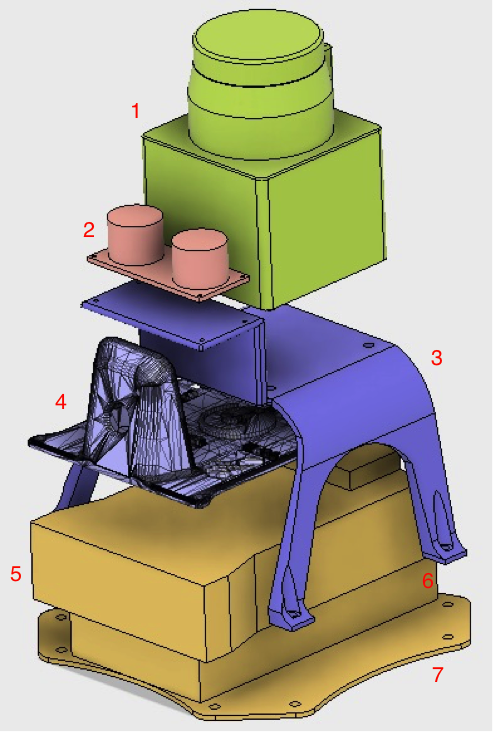
\includegraphics[width=0.7\textwidth]{imgs/mount1_labelled.png}
    \caption{First iteration, dual laser scanner and ultrasonic mount. (1) Hokuyo URG01 (2) Ultrasonic module (3) Laser scanner mount designed by URSA (4) Mesh of Erle brain lid (5) Erle brain (6) Anti-vibration bed (7) Erle copter top mounting plate.\label{fig:mount1}}
\end{figure}

\subsection{Ultrasonic Mount - Version 1}

The first iteration worked as a laser mount but did not allow for an ultrasonic component to be mounted facing the ground.  Taking range measurements from the drone to the floor were considered more reliable.  The ground is more likely to be a uniform surface, especially in emergency situations where the roof may have collapsed or wires/debris are hanging from the ceiling.  Furthermore, measurements are noisier with increased distance to reflective surface.  For our initial prototype the drone is likely to be closer to the ground than the ceiling in most situations.  As a result the ultrasonic mount was moved to the back of the landing legs.  In this position placement of upwards and downwards facing modules is possible.

\begin{figure}[H]
    \centering
    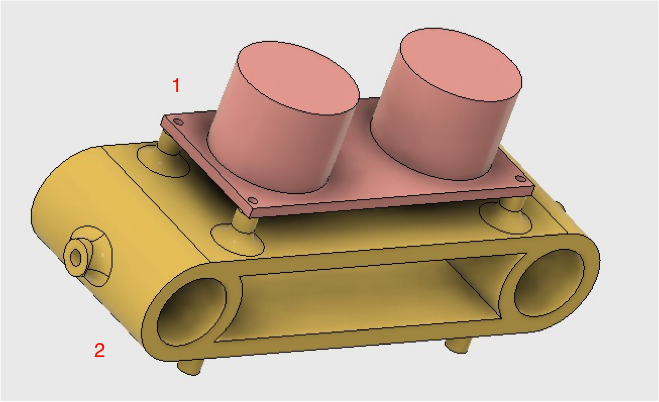
\includegraphics[width=0.6\textwidth]{imgs/mount2_labelled.png}
    \caption{Second mount design allowing for top and bottom ultrasonic mounts. (1) Ultrasonic module (2) Mount design by URSA.\label{fig:mount2}}
\end{figure}

\subsection{Ultrasonic Mount - Version 2}

The first version of ultrasonic mount fit the landing legs of the drone and ultrasonic component.  However, due to the component being used it was difficult to find screws small enough to secure the module.  Given on campus 3D printing facilities, creating an updated model to remove the need for screws was the most time efficient design decision.  The side mounting screw fitting were also removed, the tight fit of the mount to the legs meant no additional securing was necessary.

\begin{figure}[H]
    \centering
    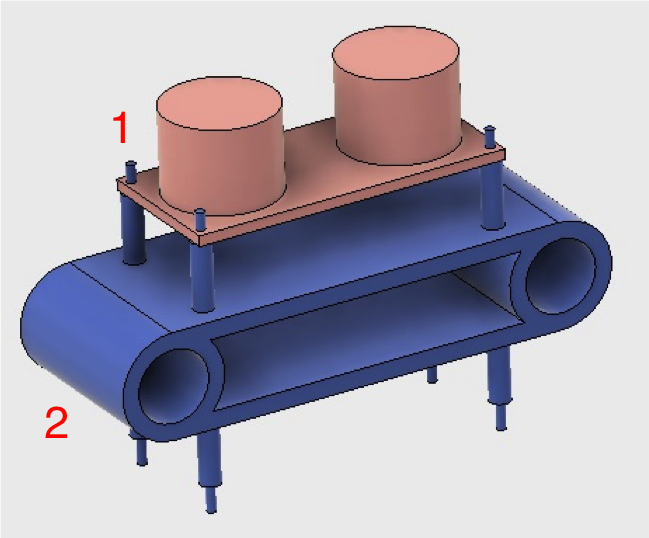
\includegraphics[width=0.6\textwidth]{imgs/mount3_labelled.png}
    \caption{Third mount deign obviating need for screws. (1) Through-hole pins (2) Removed side screw fittings. \label{fig:mount3}}
\end{figure}

\subsection{Final Mounts}

Figure \ref{fig:final_mounts} shows the final printed mounts.

\begin{figure}[H]
    \centering
    \includegraphics[width=0.7\textwidth]{example-image-a}
    \caption{Final protoypes\label{fig:final_mounts}}
\end{figure}

\section{Development of simulation environment}
\textbf{To be completed}

\section{Interfacing with sensors}
    With the Erle-Copter fully constructed, we were able to undertake some test flights as described in the previous section. However, as expected, the test flight using APM as the flight controller exhibited some drift over time. Manual correction was required by a pilot holding a remote control. The reason for this has already been discussed in previous sections - without a direct measurement of position, the system must resort to `dead-reckoning', which consists of integrating acceleration readings over time. This accumulates error, so the controller cannot hold its position. The solution to this is to replace the APM controller (provided by default with the Erle-Copter) with a PX4 controller. The PX4 controller can ingest positional information from an external source. Fusing this information with the acceleration information will provide URSA with an accurate view of its own position.\\

    The next stage of the project was therefore to build a reliable interface between PX4 and the sensors which would use the PX4 bus. Once this has been achieved, we can replace the default APM flight controller with our version of PX4. In addition to expanding the PX4 code base to deal with our sensors, there are some additional considerations and issues which will be addressed in this section: 
    \begin{itemize}
        \item Choice and implementation of operating system to support PX4 sensor polling at required latencies.
        \item Hardware based signal conditioning of the SONAR output signal.
    \end{itemize}

    Note that interfacing with the LiDAR scanner will not be discussed in this section, since this is achieved within the ROS bus, rather than the PX4 bus. This aspect of the project will be discussed in the following section.\\

    \subsection{Raspberry Pi real-time operating system}
    When writing `bare-metal' code or programming for a microcontroller, it is safe to make various assumptions about timing. For example, if we were using an STM32 ARM microcontroller, and we recieved an interrupt signal, the time taken to respond to this signal would be deterministic and probably also very fast. It is important in time-critical systems such as URSA to have upper bounds on these response times. Clearly, if there is too long of a delay between a stimulus and an actuator response, the flight system could become unstable with no prospect of recovery. \\

    When writing a program designed to be executed within an operating system, this is not the case. Software executed on an operating system typically only has access to its own address space. Interacting with resources outside of this address space (for example, writing or reading from an I2C port) is accomplished by making a `system call' to the operating system. The operating system needs to manage the external resource requirements of many different applications running concurrently, as well as its own overhead. For example, many operating systems will disable interrupts during critical system tasks. It is impossible for an application to be confident that interrupts are available at any given time. Therefore, there is no guarantee that accessing an external resource, or being triggered by an external interrupt, will happen within any specific timeframe. This is a big problem for URSA, which has critical timing requirements in ensuring flight stability.\\

    Many embedded applications share this issue, however the resource management provided by an operating system is generally desirable for complex systems. In recognition of this, a class of operating systems known as `Real-time' operating systems (RTOS) was developed. An RTOS is designed with reliable interrupts in mind. The basic idea is that no program may disable interrupts, and even the most sensitive parts of the operating system must be designed in a way which supports being interrupted. This means that the only remaining variable in the time taken for an interrupt to be serviced is the priority of a process, and the number of other processes of equal or higher priority.\\

    An example of an RTOS in use today is the Real-time Executive for Multiprocessor Systems (RTEMS)\footnote{\url{https://www.rtems.org/}}, which was originally developed for missile systems in the late 1980s. While a fully real-time OS may seem desirable for URSA, it must be weighed against the time taken to invest in developing for such a system. Ideally, we want an operating system which the main applications which form part of URSA (PX4 and ROS) can be compiled. This restricts us to a Linux based OS. Further, since we are using a Raspberry Pi it is desirable to use the default distribution from the Raspberry Pi foundation, Raspbian, since it comes with many tools and utilities for the Raspberry Pi. Raspbian does not have RTOS capabilities.\\

    Fortunately, there is a project within the Linux ecosystem known as \texttt{CONFIG\_PREEMPT\_RT}. This project is a patch which can be applied to modify the source code of the Linux kernel to support fully real-time capabilities. After applying this patch to the Linux kernel source code, we can compile this kernel and replace the default Raspbian kernel with our real-time variant. This will allow the Raspberry Pi to respond to interrupts with an acceptable level of reliability to control a flight platform in real-time.\\

    To compile the Linux kernel, we used the cross-compile tools provided by the Raspberry Pi foundation. This allowed us to compile the kernel on a desktop machine, despite the target platform being a 32-bit ARM processor. This significantly sped up the process. After cloning the Raspbian fork of the Linux kernel\footnote{Found at \url{https://github.com/raspberrypi/linux}}, we applied the \texttt{CONFIG\_PREEMPT\_RT} patch and enabled the fully pre-emptable kernel. We then built the kernel using the traditional Linux build process and GCC, having selected to cross compile for ARM 32 HF architecture.\\

    We replaced the existing kernel on our Raspbian system under \texttt{/boot} with the outputs from the above process. The system would boot, however it was observed that the Raspberry Pi would occasionally crash and need to be rebooted. After some debugging effort, it was found that these crashes were due to transferring data over the USB port. Further research \footnote{See \url{https://www.osadl.org/Single-View.111+M5c03315dc57.0.html}} led to the discovery that the problem was due to the implementation of a class of interrupts by the default Raspbian USB host driver. These interrupts are known as `fast interrupt requests' (FIQ) and operate at a higher priority to standard interrupt requests (IRQ). The problem was occuring when the IRQ thread was interrupted whilst holding the FIQ spinlock. Since the spinlock was then never released, generating an FIQ leads to an infinite loop waiting for the spin lock to be released. \\

    A simple workaround is to disable the FIQ capabilities of the USB driver. This was undertaken and provided good stability. The drawback is that USB data transfers now happen at a lower priority - however since we have minimal data requirements on the USB hub this will not be a problem for URSA. FIQ capabilities for the DWC USB controller may be disabled by adding \texttt{dwc\_otg.fiq\_enable=0 dwc\_otg.fiq\_fsm\_enable=0} to the file \texttt{/boot/cmdline.txt}. This file is run by the kernel for configuration when the system boots.\\

    Having compiled our own Linux kernel, it is beneficial to benchmark the improvement in latency in using the real-time patch. As can be seen in Figure \ref{fig:PX4Arch}, some aspects of the PX4 flight controller require sensor readings at up to \SI{8}{\kilo\hertz}. Therefore, ideally we can achieve response times under \SI{125}{\micro\second} in order to support these components\footnote{In reality, PX4 can be configured to operate at slower speeds - however this is still a reasonable target to ensure stable flight}. Benchmarking has been performed using the utility \texttt{cyclictest} with results shown in a histogram at Figure \ref{fig:RT_bench}.

    \begin{figure}[H]
        \centering
        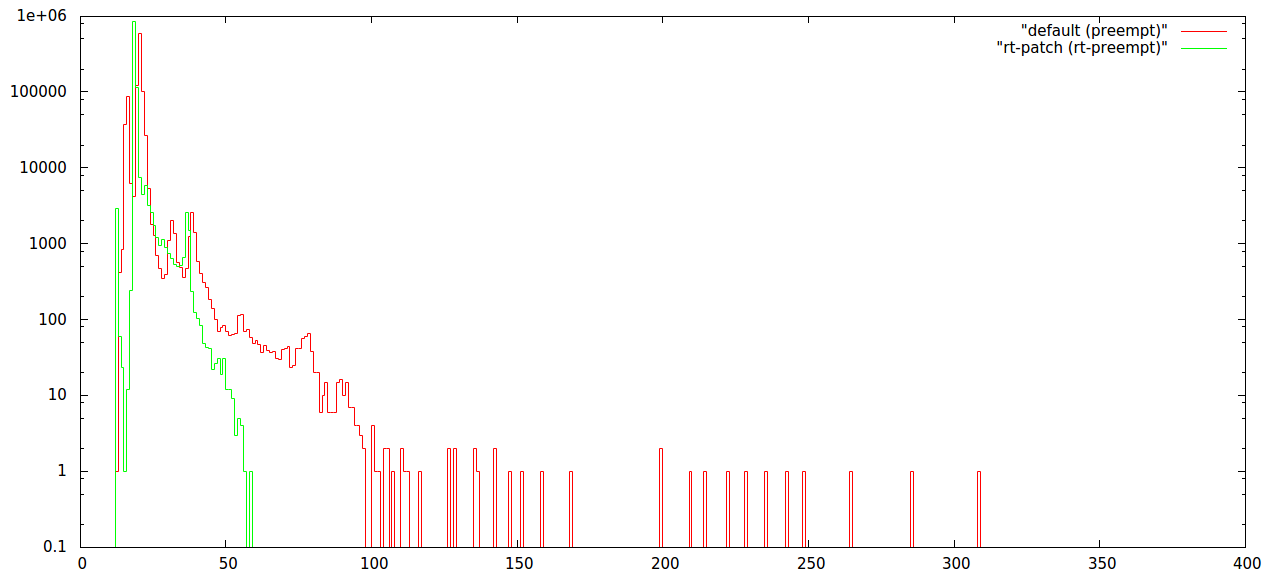
\includegraphics[width=0.8\textwidth]{imgs/rpi2-cyclictest-plot.png}
        \caption{Latency of Raspberry Pi with real-time patch(TO BE REPLACED WITH OUR OWN BENCHMARKS)\label{fig:RT_bench}}
    \end{figure}

    As can be seen, there is a significant improvement observed in latency by applying the RT patch. We are reliably getting below \SI{100}{\micro\second} in response times, whereas previously we could expect over \SI{300}{\micro\second} depending on other tasks being performed by the OS. Our new kernel is therefore more appropriate for running PX4.

    \subsection{Signal conditioning of SONAR}
 	The HC-SR04 has a very simple pulse width output, where the output of a pulse on one of the pins is proportional to the distance measured. This is shown at Figure \ref{fig:sr04}.

    \begin{figure}[H]
        \centering
        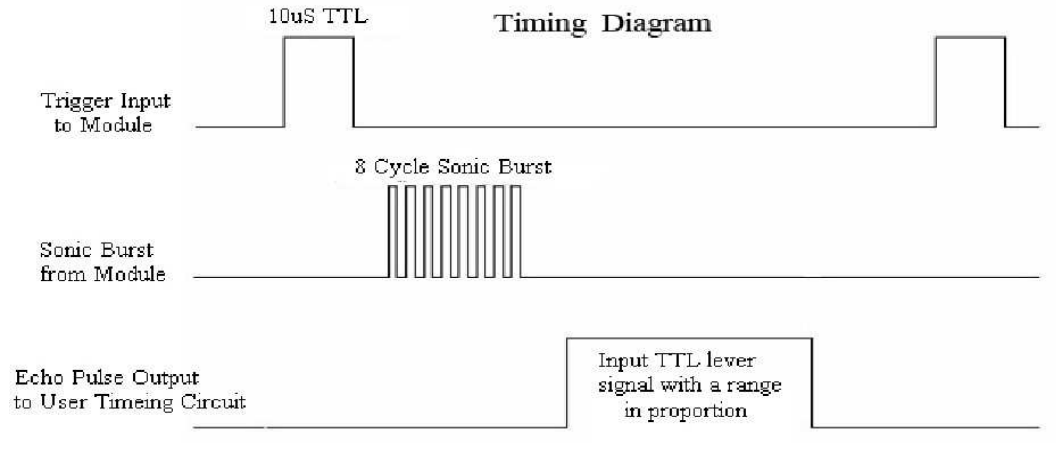
\includegraphics[width=0.8\textwidth]{imgs/sr04.png}
        \caption{HC-SR04 timing\label{fig:sr04}}
    \end{figure}

After preliminary tests, it was found that there were fluctuations in UAV altitude readings, despite no visible jump even with the UAV held at a fixed altitude. This was further investigated via an oscilloscope. It was discovered that signals on the HC-SR04 echo pin occasionally experienced voltage drops. Additional impedances and noise introduced by the wires connecting the Raspberry Pi trigger/echo pins to the HC-SR04 were hypothesised to be the cause of the issue. \\

The problem is shown at Figure \ref{fig:badSig}, where URSA was held at a fixed height and a number of measurements were overlayed on each other. As can be seen, the pulse width is not constant between subsequent measurements, as should be the case.
    \begin{figure}[H]
        \centering
        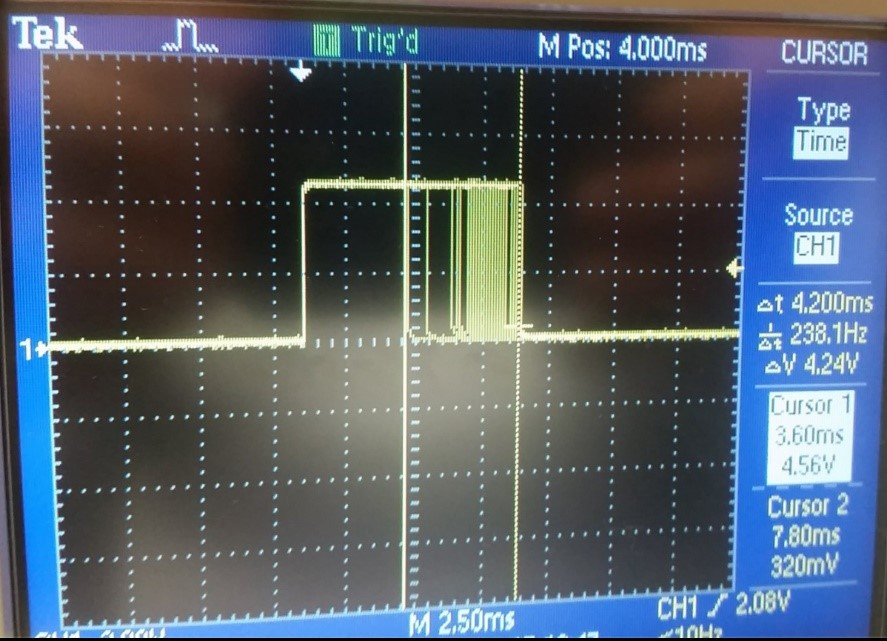
\includegraphics[width=0.8\textwidth]{imgs/pulseBroad.jpg}
        \caption{Amalgamation of sensor readings from a single height\label{fig:badSig}}
    \end{figure}

As seen in Figure \ref{fig:badSig}, the fluctuation in pulse length experienced is approximately 3.2ms, corresponding to 0.578m variation in measured distances; a clearly unacceptable figure. This is derived from first noting the speed of sound is approximately \SI{340}{\metre\per\second}, so we have the time taken, $t$, for the sound to transmit and return a distance $x$:

\begin{align*}
	x=\frac{340t}{2}
\end{align*}

It was proposed that a filter/buffer PCB could be used to remove the erroneous signals, by both restoring the integrity of any damaged signals during transmission, and filtering any rapid changes. The final schematic consists of a comparator and linear regulator to ensure that voltage supplied to the Raspberry Pi GPIO did not exceed its \SI{3.3}{\volt} limits. This is shown at Figure \ref{fig:sigSchem}.

    \begin{figure}[H]
        \centering
        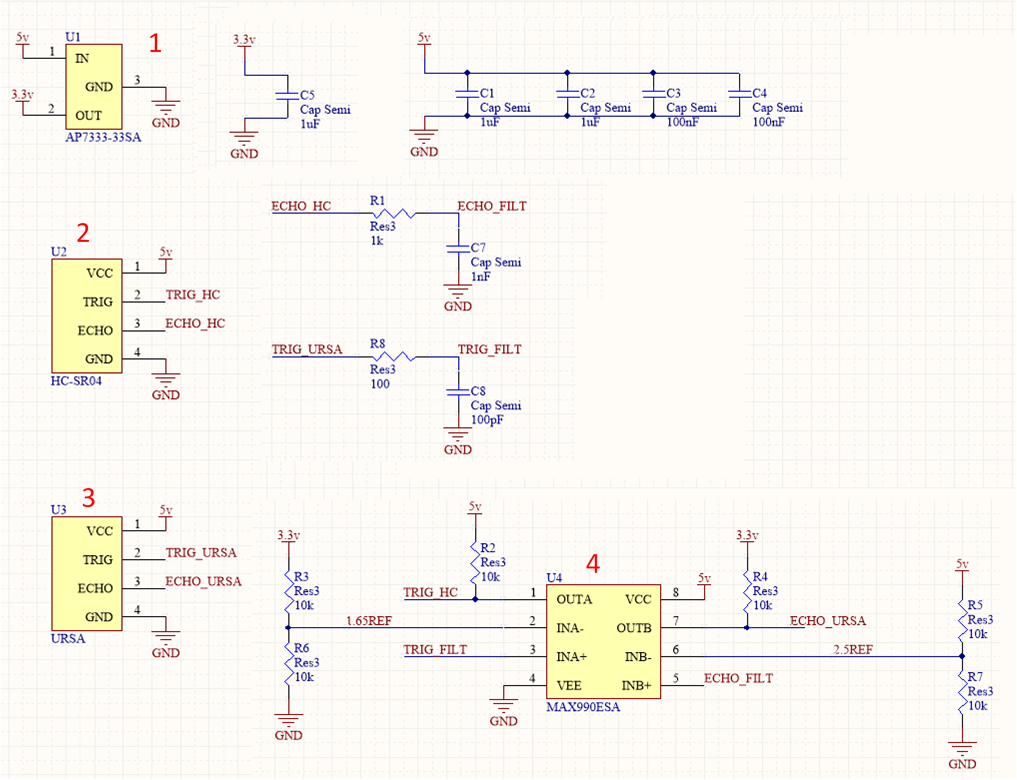
\includegraphics[width=0.8\textwidth]{imgs/schematic.png}
        \caption{Schematic for hardware signaal conditioner\label{fig:sigSchem}}
    \end{figure}

We had this PCB fabricated and assembled. This led to significantly improved results. The waveform after hardware signal conditioning is shown at Figure \ref{fig:goodSig}. As can be seen, the jitter is reduced to a negligible amount.

    \begin{figure}[H]
        \centering
        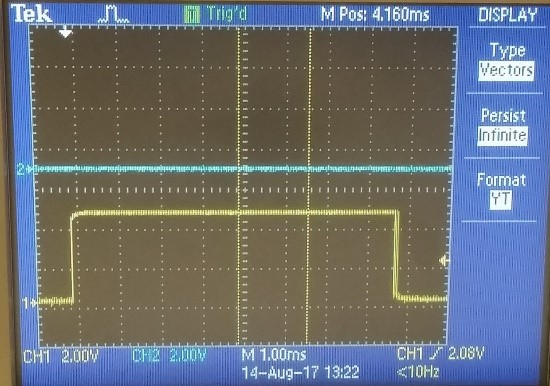
\includegraphics[width=0.8\textwidth]{imgs/pulseOk.jpg}
        \caption{Amalgamation of sensor readings from a single height\label{fig:goodSig}}
    \end{figure}

Unfortunately, we did find that starting the motors re-introduced some minor jitter. We confirmed that this wasnt due to power supply issues. It appears likely that it is due to mechanical reasons - i.e. the rotors of the drone shake the connectors to the SONAR unit. Nevertheless, results were within acceptable limits for flying and testing the prototype unit.


    \subsection{Sensor interface to PX4}
    There are two categories of sensors which were required to be interfaced with PX4. The first was the sensors provided with the Erle-copter. These sensors were mounted on a PCB which sits on top of the Raspberry Pi (the `Erle-brain'). The second category of sensors were additional sensors provided for the URSA project. The only one of these which was required to have a PX4 driver written for it was the SONAR driver.\\

    Before embarking on the full development of a driver suite to allow PX4 to access the sensor data from the Erle-Brain, we consulted the manufacturer to determine whether these were already available. The default software does ship with a closed-source version of PX4; however we found that this version was unsuitable for our requirements, both because it was closed source (and therefore precluded some of the customization and development required later in the project) and because it did not include drivers for many of the Erle-brain devices (including the ADC used to detect battery level).\\

    We queried this on the Erle-copter forums\footnote{\url{http://forum.erlerobotics.com/t/px4-on-eb3-access-to-drivers/2711}}, where it was confirmed that Erle Robotics do not provide PX4 source code. We therefore committed to building our own version of PX4 to support the hardware we had available.\\

    In order to build PX4 drivers for new hardware, there are two aspects which need to be understood in detail:
    \begin{itemize}
        \item The framework used by PX4 to interact with hardware; and,
        \item The physical layout and specifications of each hardware component.
    \end{itemize}

    Understanding the first point allows us to easily integrate our drivers with existing PX4 code; understanding the second point is necessary in designing the drivers themselves.\\

    \subsubsection{PX4 Driver Framework}
    PX4 has a specialised framework designed to allow abstraction and unification of drivers. This is called the `DriverFramework'. Some of the advantages of using DriverFramework are as follows:
    \begin{itemize}
        \item It has base classes for both I2C and SPI, including implementations of the basic IO methods required to interface over these protocols.
        \item It has been thoroughly tested on POSIX systems including for Raspberry Pi.
        \item There are defined methods for setting up drivers, allocating resources, and cleaning up. These methods are called as required by the DriverFramework.
        \item There are abstracted read/write methods which can be called simply by retrieving a handle to a driver. Handles can be acquired by using strings in the same format as a file system driver (e.g. `/dev/baro0' for a barometer).
    \end{itemize}

    More information on the DriverFramework can be found at \url{https://dev.px4.io/en/middleware/drivers.html}. The basic design pattern requires calling various initialization methods on the driver. Once the driver is initialized and started, the framework will regularly call the \texttt{\_measure} method at the specified rate. This method can publish to \texttt{uORB} topics. Additionally, other parts of the PX4 code can obtain a handle to the driver and execute \texttt{read} and \texttt{write} methods on the driver. \\

    For our PX4 drivers, we follow the design pattern of providing a PX4 wrapper application which starts and stops each of our drivers. These wrappers are called by PX4 on startup, as specified in the PX4 configuration file. The source for these wrappers are located under \texttt{Firmware/src/platforms/posix/drivers}. The drivers themselves are written and contained within the DriverFramework, under \texttt{Firmware/src/lib/DriverFramework/drivers}. Note that all PX4 code for URSA is available on GitHub at \url{https://github.com/ursa-drone/Firmware}.

    \subsubsection{Hardware review}
    Having briefly considered the software framework in which our drivers will operate, we now look at the hardware for which drivers will be required. The main piece of hardware for which drivers are required is the Erle-Brain. This is a PCB with a number of chips relevant for flight sensing and control. It is designed to attach to the top of a Raspberry Pi, as a `hat'. It is shown at Figure \ref{fig:erleHat}, with points of interest numbered. In this Figure, it can be seen mounted on top of a Raspberry Pi.

    \begin{figure}[H]
        \centering
        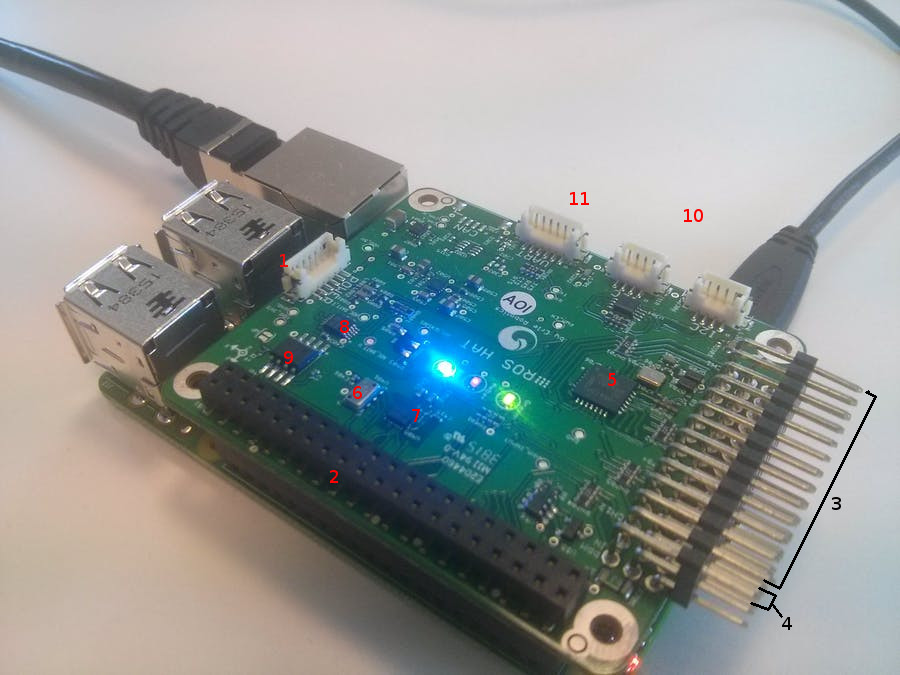
\includegraphics[width=0.8\textwidth]{imgs/erleHat.jpg}
        \caption{Erle-Brain for Raspberry Pi\label{fig:erleHat}}
    \end{figure}


    Unfortunately, Erle Robotics does not provide documentation for the devices on the Erle-brain. We were required to reverse engineer this board in order to determine the devices, functions, and connections to the Pi for each component. This consisted of physically inspecting the component packages and PCB traces in order to determine the part numbers and connections. Our findings are shown at Table \ref{tab:ebcomponents}.

    \begin{table}[H]
    \centering
        \begin{tabular}{|c|c|c|c|}
            \hline
            Reference on Figure \ref{fig:erleHat} & Description & Part number & Connection to Pi\\
            \hline
            1 & Power input & N/A & Via power pins \\
            2 & Raspberry Pi header & N/A & Direct \\
            3 & PWM Output pins & N/A & Connected to PWM controller \\
            4 & GPIO pin for RC input & N/A & GPIO 7 \\
            5 & PWM Controller & PCA9685 & I2C bus \\
            6 & Barometer & MS5611 & SPI bus using CE0 for chip select\\
            7 & Inertial measurement unit & MPU9250 & SPI bus using CE1 for chip select\\
            8 & ADC for battery life & ADS1115 & I2C bus \\
            9 & EEPROM - see below & N/A & ID\_SC and ID\_SD pins\\
            10 & I2C bus outputs & N/A & I2C bus \\
            11 & UART output & N/A & UART \\
            \hline
        \end{tabular}
    \caption{Components on Erle-brain\label{tab:ebcomponents}}
    \end{table}

    In relation to the EERPOM component, we note that this is a requirement of so-called standardised `hats' for Raspberry Pi. Each hat requires an EEPROM module which contains information about the connected component, connected to reserved pins on the Pi. This is meant to allow easier software implementation of drivers; however in our case we found that the EEPROM on the Erle-brain had no useful information. It was therefore ignored for this project.\\

    In relation to the PWM chip, it may seem strange at first to have this device on the Erle-brain. After all, we do have a Raspberry Pi with a PWM output. The reason it is present is that it uses its own crystal, visible on Figure \ref{fig:erleHat}, to achieve significantly faster PWM frequencies than can be delivered by the Pi. It also frees up resources on the Pi. Finally, the Pi only has a single hardware PWM output port. We require at least four PWM outputs (one for each motor). Using a dedicated PWM chip is therefore the correct design pattern.

    \subsubsection{Development of drivers for I2C \& SPI components}
    As can be seen in Table \ref{tab:ebcomponents}, four of the components on the Erle-Brain interact via relatively simple I2C/SPI protocols. As mentioned previously, the PX4 DriverFramework contains parent classes for I2C and SPI components. These classes interface with the relevant components by accessing the file system components exposed by the Raspbian operating system. \\

    For example, the Raspberry Pi has a single SPI interface which supports 2 channels, on pins CE0 and CE1. The device connected to pin CE0 is exposed in the file system as \texttt{/dev/spidev0.0}. Likewise, the device on pin CE1 is exposed as texttt{/dev/spidev0.1}. These devices can be accessed using the general purpose \texttt{ioctl} system calls. The following code snippet illustrates how these devices may be accessed using system calls:

\begin{lstlisting}[language=c++]
#include <fcntl.h>
#include <sys/ioctl.h>     
#include <linux/spi/spidev.h>
#include <unistd.h>
int *spi_cs_fd;
*spi_cs_fd = open("/dev/spidev0.0", O_RDWR);
struct spi_ioc_transfer spi;
int length;
// Initialise properties of spi struct
// This includes pointer to data to write, pointer to data to read
// Initialise length
ioctl(*spi_cs_fd, SPI_IOC_MESSAGE(length), &spi);
\end{lstlisting}

    A more comprehensive version of the above code is implemented in PX4's DriverFramework, under the class SPIDevObj. A similar class exists called I2CDevObj. The main difference for this class is that an I2C address is also required to initialise this type of object. This is because while SPI uses a wire to select devices on the bus, I2C uses a code number at the beginning of the transmission. Some debugging of these base classes was required, due to our implementation on a Raspberry Pi. \\

    Using these base classes, we were able to subclass new driver classes for each of the components PCA9685, ADS1115, MS5611, and MPU9250. The driver classes contain methods which are derived from each components' datasheet. All datasheets have been included as appendices to this report. We also wrote wrappers which were able to initialise each of these classes, as mentioned previously. The source for each driver is included under the directories mentioned above.\\

    In the case of the PCA9685, this component also has an output enable pin for enabling PWM output. To control this pin, we used the GPIO driver which will be discussed below. This illustrates the power of using the PX4 DriverFramework - if any section of the code requires access to a device, it can simply request a handle to that device by name and execute read/write operations as required.

    \subsubsection{Development of GPIO drivers}
    In addition to the digital components described above, there are also two analog components within the URSA hardware ecosystem:
    \begin{itemize}
        \item The RC reciever; and,
        \item The SONAR rangefinder 
    \end{itemize}

    The operation of the SONAR rangefinder has already been discussed in-depth. The RC reciever operates on a similar principle - analog signals proportional to pulse width - however it also allows multiplexing of different channels via pulse positional modulation (PPM). In this scheme, each of the channels represents one piece of data from the remote controller. This could be the position of a switch, the position of a joystick in the x-axis, the position of a joystick in the y-axis, etc. Each of these channels can be assigned a function within PX4 once they have been decoded, such as roll, pitch, yaw, land etc.\\

    An illustration of the waveform generated by the reciever is shown at Figure \ref{fig:ppm}.

    \begin{figure}[H]
    \centering
        % Graphic for TeX using PGF
% Title: /home/lach/uni/ursa/ppm.dia
% Creator: Dia v0.97.3
% CreationDate: Mon Sep 25 17:30:06 2017
% For: lach
% \usepackage{tikz}
% The following commands are not supported in PSTricks at present
% We define them conditionally, so when they are implemented,
% this pgf file will use them.
\ifx\du\undefined
  \newlength{\du}
\fi
\setlength{\du}{15\unitlength}
\begin{tikzpicture}
\pgftransformxscale{1.000000}
\pgftransformyscale{-1.000000}
\definecolor{dialinecolor}{rgb}{0.000000, 0.000000, 0.000000}
\pgfsetstrokecolor{dialinecolor}
\definecolor{dialinecolor}{rgb}{1.000000, 1.000000, 1.000000}
\pgfsetfillcolor{dialinecolor}
\pgfsetlinewidth{0.100000\du}
\pgfsetdash{}{0pt}
\pgfsetdash{}{0pt}
\pgfsetbuttcap
{
\definecolor{dialinecolor}{rgb}{0.000000, 0.000000, 0.000000}
\pgfsetfillcolor{dialinecolor}
% was here!!!
\pgfsetarrowsend{to}
\definecolor{dialinecolor}{rgb}{0.000000, 0.000000, 0.000000}
\pgfsetstrokecolor{dialinecolor}
\draw (0.000000\du,24.000000\du)--(0.000000\du,13.000000\du);
}
\pgfsetlinewidth{0.100000\du}
\pgfsetdash{}{0pt}
\pgfsetdash{}{0pt}
\pgfsetbuttcap
{
\definecolor{dialinecolor}{rgb}{0.000000, 0.000000, 0.000000}
\pgfsetfillcolor{dialinecolor}
% was here!!!
\definecolor{dialinecolor}{rgb}{0.000000, 0.000000, 0.000000}
\pgfsetstrokecolor{dialinecolor}
\draw (0.000000\du,16.000000\du)--(-1.000000\du,16.000000\du);
}
% setfont left to latex
\definecolor{dialinecolor}{rgb}{0.000000, 0.000000, 0.000000}
\pgfsetstrokecolor{dialinecolor}
\node[anchor=west] at (-2.000000\du,16.000000\du){5v};
\pgfsetlinewidth{0.100000\du}
\pgfsetdash{}{0pt}
\pgfsetdash{}{0pt}
\pgfsetbuttcap
{
\definecolor{dialinecolor}{rgb}{0.093248, 0.027771, 0.978149}
\pgfsetfillcolor{dialinecolor}
% was here!!!
\definecolor{dialinecolor}{rgb}{0.093248, 0.027771, 0.978149}
\pgfsetstrokecolor{dialinecolor}
\draw (0.000000\du,16.000000\du)--(2.000000\du,16.000000\du);
}
\pgfsetlinewidth{0.100000\du}
\pgfsetdash{}{0pt}
\pgfsetdash{}{0pt}
\pgfsetbuttcap
{
\definecolor{dialinecolor}{rgb}{0.093248, 0.027771, 0.978149}
\pgfsetfillcolor{dialinecolor}
% was here!!!
\definecolor{dialinecolor}{rgb}{0.093248, 0.027771, 0.978149}
\pgfsetstrokecolor{dialinecolor}
\draw (2.000000\du,16.000000\du)--(2.000000\du,24.000000\du);
}
\pgfsetlinewidth{0.100000\du}
\pgfsetdash{}{0pt}
\pgfsetdash{}{0pt}
\pgfsetbuttcap
{
\definecolor{dialinecolor}{rgb}{0.093248, 0.027771, 0.978149}
\pgfsetfillcolor{dialinecolor}
% was here!!!
\definecolor{dialinecolor}{rgb}{0.093248, 0.027771, 0.978149}
\pgfsetstrokecolor{dialinecolor}
\draw (2.000000\du,24.000000\du)--(3.000000\du,24.000000\du);
}
\pgfsetlinewidth{0.100000\du}
\pgfsetdash{}{0pt}
\pgfsetdash{}{0pt}
\pgfsetbuttcap
{
\definecolor{dialinecolor}{rgb}{0.093248, 0.027771, 0.978149}
\pgfsetfillcolor{dialinecolor}
% was here!!!
\definecolor{dialinecolor}{rgb}{0.093248, 0.027771, 0.978149}
\pgfsetstrokecolor{dialinecolor}
\draw (3.000000\du,24.000000\du)--(3.000000\du,16.000000\du);
}
\pgfsetlinewidth{0.100000\du}
\pgfsetdash{}{0pt}
\pgfsetdash{}{0pt}
\pgfsetbuttcap
{
\definecolor{dialinecolor}{rgb}{0.093248, 0.027771, 0.978149}
\pgfsetfillcolor{dialinecolor}
% was here!!!
\definecolor{dialinecolor}{rgb}{0.093248, 0.027771, 0.978149}
\pgfsetstrokecolor{dialinecolor}
\draw (3.000000\du,16.000000\du)--(8.000000\du,16.000000\du);
}
\pgfsetlinewidth{0.100000\du}
\pgfsetdash{}{0pt}
\pgfsetdash{}{0pt}
\pgfsetbuttcap
{
\definecolor{dialinecolor}{rgb}{0.093248, 0.027771, 0.978149}
\pgfsetfillcolor{dialinecolor}
% was here!!!
\definecolor{dialinecolor}{rgb}{0.093248, 0.027771, 0.978149}
\pgfsetstrokecolor{dialinecolor}
\draw (8.000000\du,16.000000\du)--(8.000000\du,24.000000\du);
}
\pgfsetlinewidth{0.100000\du}
\pgfsetdash{}{0pt}
\pgfsetdash{}{0pt}
\pgfsetbuttcap
{
\definecolor{dialinecolor}{rgb}{0.093248, 0.027771, 0.978149}
\pgfsetfillcolor{dialinecolor}
% was here!!!
\definecolor{dialinecolor}{rgb}{0.093248, 0.027771, 0.978149}
\pgfsetstrokecolor{dialinecolor}
\draw (8.000000\du,24.000000\du)--(9.000000\du,24.000000\du);
}
\pgfsetlinewidth{0.100000\du}
\pgfsetdash{}{0pt}
\pgfsetdash{}{0pt}
\pgfsetbuttcap
{
\definecolor{dialinecolor}{rgb}{0.093248, 0.027771, 0.978149}
\pgfsetfillcolor{dialinecolor}
% was here!!!
\definecolor{dialinecolor}{rgb}{0.093248, 0.027771, 0.978149}
\pgfsetstrokecolor{dialinecolor}
\draw (9.000000\du,24.000000\du)--(9.000000\du,16.000000\du);
}
\pgfsetlinewidth{0.100000\du}
\pgfsetdash{}{0pt}
\pgfsetdash{}{0pt}
\pgfsetbuttcap
{
\definecolor{dialinecolor}{rgb}{0.093248, 0.027771, 0.978149}
\pgfsetfillcolor{dialinecolor}
% was here!!!
\definecolor{dialinecolor}{rgb}{0.093248, 0.027771, 0.978149}
\pgfsetstrokecolor{dialinecolor}
\draw (9.000000\du,16.000000\du)--(12.000000\du,16.000000\du);
}
\pgfsetlinewidth{0.100000\du}
\pgfsetdash{}{0pt}
\pgfsetdash{}{0pt}
\pgfsetbuttcap
{
\definecolor{dialinecolor}{rgb}{0.093248, 0.027771, 0.978149}
\pgfsetfillcolor{dialinecolor}
% was here!!!
\definecolor{dialinecolor}{rgb}{0.093248, 0.027771, 0.978149}
\pgfsetstrokecolor{dialinecolor}
\draw (12.000000\du,16.000000\du)--(12.000000\du,16.000000\du);
}
\pgfsetlinewidth{0.100000\du}
\pgfsetdash{}{0pt}
\pgfsetdash{}{0pt}
\pgfsetbuttcap
{
\definecolor{dialinecolor}{rgb}{0.093248, 0.027771, 0.978149}
\pgfsetfillcolor{dialinecolor}
% was here!!!
\definecolor{dialinecolor}{rgb}{0.093248, 0.027771, 0.978149}
\pgfsetstrokecolor{dialinecolor}
\draw (12.000000\du,16.000000\du)--(12.000000\du,24.000000\du);
}
\pgfsetlinewidth{0.100000\du}
\pgfsetdash{}{0pt}
\pgfsetdash{}{0pt}
\pgfsetbuttcap
{
\definecolor{dialinecolor}{rgb}{0.093248, 0.027771, 0.978149}
\pgfsetfillcolor{dialinecolor}
% was here!!!
\definecolor{dialinecolor}{rgb}{0.093248, 0.027771, 0.978149}
\pgfsetstrokecolor{dialinecolor}
\draw (13.000000\du,24.000000\du)--(13.000000\du,24.000000\du);
}
\pgfsetlinewidth{0.100000\du}
\pgfsetdash{}{0pt}
\pgfsetdash{}{0pt}
\pgfsetbuttcap
{
\definecolor{dialinecolor}{rgb}{0.093248, 0.027771, 0.978149}
\pgfsetfillcolor{dialinecolor}
% was here!!!
\definecolor{dialinecolor}{rgb}{0.093248, 0.027771, 0.978149}
\pgfsetstrokecolor{dialinecolor}
\draw (18.000000\du,24.000000\du)--(18.000000\du,16.000000\du);
}
\pgfsetlinewidth{0.100000\du}
\pgfsetdash{}{0pt}
\pgfsetdash{}{0pt}
\pgfsetbuttcap
{
\definecolor{dialinecolor}{rgb}{0.093248, 0.027771, 0.978149}
\pgfsetfillcolor{dialinecolor}
% was here!!!
\definecolor{dialinecolor}{rgb}{0.093248, 0.027771, 0.978149}
\pgfsetstrokecolor{dialinecolor}
\draw (18.000000\du,16.000000\du)--(20.000000\du,16.000000\du);
}
% setfont left to latex
\definecolor{dialinecolor}{rgb}{0.000000, 0.000000, 0.000000}
\pgfsetstrokecolor{dialinecolor}
\node[anchor=west] at (9.000000\du,15.000000\du){Channel N};
% setfont left to latex
\definecolor{dialinecolor}{rgb}{0.000000, 0.000000, 0.000000}
\pgfsetstrokecolor{dialinecolor}
\node[anchor=west] at (3.000000\du,15.000000\du){Channel N-1};
% setfont left to latex
\definecolor{dialinecolor}{rgb}{0.000000, 0.000000, 0.000000}
\pgfsetstrokecolor{dialinecolor}
\node[anchor=west] at (0.000000\du,15.000000\du){...};
% setfont left to latex
\definecolor{dialinecolor}{rgb}{0.000000, 0.000000, 0.000000}
\pgfsetstrokecolor{dialinecolor}
\node[anchor=west] at (18.000000\du,15.000000\du){Channel 1};
\pgfsetlinewidth{0.100000\du}
\pgfsetdash{}{0pt}
\pgfsetdash{}{0pt}
\pgfsetbuttcap
{
\definecolor{dialinecolor}{rgb}{0.000000, 0.000000, 0.000000}
\pgfsetfillcolor{dialinecolor}
% was here!!!
\pgfsetarrowsstart{latex}
\pgfsetarrowsend{latex}
\definecolor{dialinecolor}{rgb}{0.000000, 0.000000, 0.000000}
\pgfsetstrokecolor{dialinecolor}
\draw (3.000000\du,15.500000\du)--(8.000000\du,15.500000\du);
}
\pgfsetlinewidth{0.100000\du}
\pgfsetdash{}{0pt}
\pgfsetdash{}{0pt}
\pgfsetbuttcap
{
\definecolor{dialinecolor}{rgb}{0.000000, 0.000000, 0.000000}
\pgfsetfillcolor{dialinecolor}
% was here!!!
\pgfsetarrowsstart{latex}
\pgfsetarrowsend{latex}
\definecolor{dialinecolor}{rgb}{0.000000, 0.000000, 0.000000}
\pgfsetstrokecolor{dialinecolor}
\draw (9.000000\du,15.500000\du)--(12.000000\du,15.500000\du);
}
\pgfsetlinewidth{0.100000\du}
\pgfsetdash{}{0pt}
\pgfsetdash{}{0pt}
\pgfsetbuttcap
{
\definecolor{dialinecolor}{rgb}{0.000000, 0.000000, 0.000000}
\pgfsetfillcolor{dialinecolor}
% was here!!!
\pgfsetarrowsstart{latex}
\pgfsetarrowsend{latex}
\definecolor{dialinecolor}{rgb}{0.000000, 0.000000, 0.000000}
\pgfsetstrokecolor{dialinecolor}
\draw (12.000000\du,22.000000\du)--(18.000000\du,22.000000\du);
}
% setfont left to latex
\definecolor{dialinecolor}{rgb}{0.000000, 0.000000, 0.000000}
\pgfsetstrokecolor{dialinecolor}
\node[anchor=west] at (13.000000\du,20.000000\du){Break for new };
% setfont left to latex
\definecolor{dialinecolor}{rgb}{0.000000, 0.000000, 0.000000}
\pgfsetstrokecolor{dialinecolor}
\node[anchor=west] at (13.000000\du,20.800000\du){frame};
% setfont left to latex
\definecolor{dialinecolor}{rgb}{0.000000, 0.000000, 0.000000}
\pgfsetstrokecolor{dialinecolor}
\node[anchor=west] at (20.000000\du,24.000000\du){Time};
% setfont left to latex
\definecolor{dialinecolor}{rgb}{0.000000, 0.000000, 0.000000}
\pgfsetstrokecolor{dialinecolor}
\node[anchor=west] at (-2.000000\du,24.000000\du){0v};
\pgfsetlinewidth{0.100000\du}
\pgfsetdash{}{0pt}
\pgfsetdash{}{0pt}
\pgfsetbuttcap
{
\definecolor{dialinecolor}{rgb}{0.000000, 0.000000, 0.000000}
\pgfsetfillcolor{dialinecolor}
% was here!!!
\definecolor{dialinecolor}{rgb}{0.000000, 0.000000, 0.000000}
\pgfsetstrokecolor{dialinecolor}
\draw (0.000000\du,24.000000\du)--(-1.000000\du,24.000000\du);
}
\pgfsetlinewidth{0.100000\du}
\pgfsetdash{}{0pt}
\pgfsetdash{}{0pt}
\pgfsetbuttcap
{
\definecolor{dialinecolor}{rgb}{0.000000, 0.000000, 0.000000}
\pgfsetfillcolor{dialinecolor}
% was here!!!
\pgfsetarrowsend{to}
\definecolor{dialinecolor}{rgb}{0.000000, 0.000000, 0.000000}
\pgfsetstrokecolor{dialinecolor}
\draw (0.000000\du,24.000000\du)--(20.000000\du,24.000000\du);
}
\end{tikzpicture}

        \caption{PPM illustration\label{fig:ppm}}
    \end{figure}

    The frame duration for PPM is approximately \SI{20}{\milli\second}, with each channel having a duration of between \SI{0.7}{\milli\second} to \SI{2.3}{\milli\second}. A channel pulse duration of \SI{1.5}{\milli\second} indicates a neutral value, for example a joystick at the center. To decode this signal, we need fast, regular sampling of the GPIO pin. We will need this same mechanism for the SONAR pin, so it is worth writing a general purpose fast GPIO driver which can be used by both of these other drivers (as well as the PCA9685 as mentioned above).\\

    The standard method of accessing the Raspberry Pi GPIO pins is through the Raspbian operating system. Pins can be exposed as file system objects, and written to/read from in a similar way to the SPI/I2C drivers mentioned above. However, by consulting Figure \ref{fig:RT_bench}, we can see that even with our real-time operating system, we can probably only expect to be sampling the GPIO every \SI{100}{\micro\second}. For a pulse with a range of \SI{1600}{\micro\second}, this gives us a quantization error of around 6\%. \\

    This is probably not acceptable for our purposes. In addition, since we cannot sample the GPIO at reliable intervals, we would need to also sample the clock register every sample. Further, having the CPU sample the GPIO registers so often would be very slow and likely cause issues with the other software running on the Raspberry Pi.\\

    A superior method for high frequency GPIO sampling is to swap the GPIO register into our program memory, interleaved with samples from the system clock register. This can be accomplished with only minimal CPU overhead at a very fast rate by using the direct memory access (DMA) peripheral which comes with the BCM2835 used by the Raspberry Pi. The datasheet for BCM2835 peripherals is included in the Appendices.\\

    To use the DMA capabilities, we need to provide a regular clock to trigger DMA transfers. This can be accomplished using the PCM module, also in the BCM2835 peripherals. PCM is a telephony/audio data protocol. It is possible to configure the PCM module to generate a DMA interrupt request whenever its FIFO buffer falls below a configurable level. This allows the DMA to fill up the FIFO again, ensuring uninterrupted data transfer. \\  

    In our case, we do not require the use of the Raspberry Pi's PCM capabilities. We can therefore load the PCM module with `dummy' data to initiate a transfer, and have the DMA interrupt request fire after just one bit has been transferred. This allows reliable control of the timing between successive DMA samples, at sampling times which can easily reach \SI{1}{\micro\second}. This process is shown at Figure \ref{fig:dma1}.


    \begin{figure}[H]
    \centering
        % Graphic for TeX using PGF
% Title: /home/lach/uni/ursa/DMA_1.dia
% Creator: Dia v0.97.3
% CreationDate: Mon Sep 25 18:33:41 2017
% For: lach
% \usepackage{tikz}
% The following commands are not supported in PSTricks at present
% We define them conditionally, so when they are implemented,
% this pgf file will use them.
\ifx\du\undefined
  \newlength{\du}
\fi
\setlength{\du}{15\unitlength}
\begin{tikzpicture}
\pgftransformxscale{1.000000}
\pgftransformyscale{-1.000000}
\definecolor{dialinecolor}{rgb}{0.000000, 0.000000, 0.000000}
\pgfsetstrokecolor{dialinecolor}
\definecolor{dialinecolor}{rgb}{1.000000, 1.000000, 1.000000}
\pgfsetfillcolor{dialinecolor}
\definecolor{dialinecolor}{rgb}{1.000000, 1.000000, 1.000000}
\pgfsetfillcolor{dialinecolor}
\fill (2.000000\du,10.000000\du)--(2.000000\du,13.000000\du)--(12.135000\du,13.000000\du)--(12.135000\du,10.000000\du)--cycle;
\pgfsetlinewidth{0.100000\du}
\pgfsetdash{}{0pt}
\pgfsetdash{}{0pt}
\pgfsetmiterjoin
\definecolor{dialinecolor}{rgb}{0.000000, 0.000000, 0.000000}
\pgfsetstrokecolor{dialinecolor}
\draw (2.000000\du,10.000000\du)--(2.000000\du,13.000000\du)--(12.135000\du,13.000000\du)--(12.135000\du,10.000000\du)--cycle;
% setfont left to latex
\definecolor{dialinecolor}{rgb}{0.000000, 0.000000, 0.000000}
\pgfsetstrokecolor{dialinecolor}
\node at (7.067500\du,11.295000\du){DMA Transfers GPIO register};
% setfont left to latex
\definecolor{dialinecolor}{rgb}{0.000000, 0.000000, 0.000000}
\pgfsetstrokecolor{dialinecolor}
\node at (7.067500\du,12.095000\du){into program memory};
\definecolor{dialinecolor}{rgb}{1.000000, 1.000000, 1.000000}
\pgfsetfillcolor{dialinecolor}
\fill (2.000000\du,14.000000\du)--(2.000000\du,18.000000\du)--(12.205000\du,18.000000\du)--(12.205000\du,14.000000\du)--cycle;
\pgfsetlinewidth{0.100000\du}
\pgfsetdash{}{0pt}
\pgfsetdash{}{0pt}
\pgfsetmiterjoin
\definecolor{dialinecolor}{rgb}{0.000000, 0.000000, 0.000000}
\pgfsetstrokecolor{dialinecolor}
\draw (2.000000\du,14.000000\du)--(2.000000\du,18.000000\du)--(12.205000\du,18.000000\du)--(12.205000\du,14.000000\du)--cycle;
% setfont left to latex
\definecolor{dialinecolor}{rgb}{0.000000, 0.000000, 0.000000}
\pgfsetstrokecolor{dialinecolor}
\node at (7.102500\du,15.395000\du){DMA Transfers clock register};
% setfont left to latex
\definecolor{dialinecolor}{rgb}{0.000000, 0.000000, 0.000000}
\pgfsetstrokecolor{dialinecolor}
\node at (7.102500\du,16.195000\du){into program memory};
% setfont left to latex
\definecolor{dialinecolor}{rgb}{0.000000, 0.000000, 0.000000}
\pgfsetstrokecolor{dialinecolor}
\node at (7.102500\du,16.995000\du){as a timestamp};
\definecolor{dialinecolor}{rgb}{1.000000, 1.000000, 1.000000}
\pgfsetfillcolor{dialinecolor}
\fill (2.000000\du,19.000000\du)--(2.000000\du,23.000000\du)--(12.130000\du,23.000000\du)--(12.130000\du,19.000000\du)--cycle;
\pgfsetlinewidth{0.100000\du}
\pgfsetdash{}{0pt}
\pgfsetdash{}{0pt}
\pgfsetmiterjoin
\definecolor{dialinecolor}{rgb}{0.000000, 0.000000, 0.000000}
\pgfsetstrokecolor{dialinecolor}
\draw (2.000000\du,19.000000\du)--(2.000000\du,23.000000\du)--(12.130000\du,23.000000\du)--(12.130000\du,19.000000\du)--cycle;
% setfont left to latex
\definecolor{dialinecolor}{rgb}{0.000000, 0.000000, 0.000000}
\pgfsetstrokecolor{dialinecolor}
\node at (7.065000\du,20.395000\du){DMA transfers dummy data };
% setfont left to latex
\definecolor{dialinecolor}{rgb}{0.000000, 0.000000, 0.000000}
\pgfsetstrokecolor{dialinecolor}
\node at (7.065000\du,21.195000\du){into PCM buffer and};
% setfont left to latex
\definecolor{dialinecolor}{rgb}{0.000000, 0.000000, 0.000000}
\pgfsetstrokecolor{dialinecolor}
\node at (7.065000\du,21.995000\du){enters sleep mode};
\definecolor{dialinecolor}{rgb}{1.000000, 1.000000, 1.000000}
\pgfsetfillcolor{dialinecolor}
\fill (14.000000\du,17.000000\du)--(14.000000\du,21.000000\du)--(25.240000\du,21.000000\du)--(25.240000\du,17.000000\du)--cycle;
\pgfsetlinewidth{0.100000\du}
\pgfsetdash{}{0pt}
\pgfsetdash{}{0pt}
\pgfsetmiterjoin
\definecolor{dialinecolor}{rgb}{0.000000, 0.000000, 0.000000}
\pgfsetstrokecolor{dialinecolor}
\draw (14.000000\du,17.000000\du)--(14.000000\du,21.000000\du)--(25.240000\du,21.000000\du)--(25.240000\du,17.000000\du)--cycle;
% setfont left to latex
\definecolor{dialinecolor}{rgb}{0.000000, 0.000000, 0.000000}
\pgfsetstrokecolor{dialinecolor}
\node at (19.620000\du,18.795000\du){PCM buffer generates};
% setfont left to latex
\definecolor{dialinecolor}{rgb}{0.000000, 0.000000, 0.000000}
\pgfsetstrokecolor{dialinecolor}
\node at (19.620000\du,19.595000\du){interrupt after transferring 1 bit};
\definecolor{dialinecolor}{rgb}{1.000000, 1.000000, 1.000000}
\pgfsetfillcolor{dialinecolor}
\fill (14.000000\du,12.000000\du)--(14.000000\du,16.000000\du)--(25.240000\du,16.000000\du)--(25.240000\du,12.000000\du)--cycle;
\pgfsetlinewidth{0.100000\du}
\pgfsetdash{}{0pt}
\pgfsetdash{}{0pt}
\pgfsetmiterjoin
\definecolor{dialinecolor}{rgb}{0.000000, 0.000000, 0.000000}
\pgfsetstrokecolor{dialinecolor}
\draw (14.000000\du,12.000000\du)--(14.000000\du,16.000000\du)--(25.240000\du,16.000000\du)--(25.240000\du,12.000000\du)--cycle;
% setfont left to latex
\definecolor{dialinecolor}{rgb}{0.000000, 0.000000, 0.000000}
\pgfsetstrokecolor{dialinecolor}
\node at (19.620000\du,14.195000\du){Interrupt wakes DMA};
\pgfsetlinewidth{0.100000\du}
\pgfsetdash{}{0pt}
\pgfsetdash{}{0pt}
\pgfsetmiterjoin
\pgfsetbuttcap
{
\definecolor{dialinecolor}{rgb}{0.000000, 0.000000, 0.000000}
\pgfsetfillcolor{dialinecolor}
% was here!!!
\pgfsetarrowsend{latex}
{\pgfsetcornersarced{\pgfpoint{0.000000\du}{0.000000\du}}\definecolor{dialinecolor}{rgb}{0.000000, 0.000000, 0.000000}
\pgfsetstrokecolor{dialinecolor}
\draw (19.620000\du,12.000000\du)--(19.620000\du,8.950000\du)--(7.067500\du,8.950000\du)--(7.067500\du,10.000000\du);
}}
\pgfsetlinewidth{0.100000\du}
\pgfsetdash{}{0pt}
\pgfsetdash{}{0pt}
\pgfsetbuttcap
{
\definecolor{dialinecolor}{rgb}{0.000000, 0.000000, 0.000000}
\pgfsetfillcolor{dialinecolor}
% was here!!!
\pgfsetarrowsend{latex}
\definecolor{dialinecolor}{rgb}{0.000000, 0.000000, 0.000000}
\pgfsetstrokecolor{dialinecolor}
\draw (7.067500\du,13.000000\du)--(7.102500\du,14.000000\du);
}
\pgfsetlinewidth{0.100000\du}
\pgfsetdash{}{0pt}
\pgfsetdash{}{0pt}
\pgfsetbuttcap
{
\definecolor{dialinecolor}{rgb}{0.000000, 0.000000, 0.000000}
\pgfsetfillcolor{dialinecolor}
% was here!!!
\pgfsetarrowsend{latex}
\definecolor{dialinecolor}{rgb}{0.000000, 0.000000, 0.000000}
\pgfsetstrokecolor{dialinecolor}
\draw (7.102500\du,18.000000\du)--(7.065000\du,19.000000\du);
}
\pgfsetlinewidth{0.100000\du}
\pgfsetdash{}{0pt}
\pgfsetdash{}{0pt}
\pgfsetmiterjoin
\pgfsetbuttcap
{
\definecolor{dialinecolor}{rgb}{0.000000, 0.000000, 0.000000}
\pgfsetfillcolor{dialinecolor}
% was here!!!
\pgfsetarrowsend{latex}
{\pgfsetcornersarced{\pgfpoint{0.000000\du}{0.000000\du}}\definecolor{dialinecolor}{rgb}{0.000000, 0.000000, 0.000000}
\pgfsetstrokecolor{dialinecolor}
\draw (7.065000\du,23.000000\du)--(7.065000\du,24.050000\du)--(19.620000\du,24.050000\du)--(19.620000\du,21.050250\du);
}}
\pgfsetlinewidth{0.100000\du}
\pgfsetdash{}{0pt}
\pgfsetdash{}{0pt}
\pgfsetbuttcap
{
\definecolor{dialinecolor}{rgb}{0.000000, 0.000000, 0.000000}
\pgfsetfillcolor{dialinecolor}
% was here!!!
\pgfsetarrowsend{latex}
\definecolor{dialinecolor}{rgb}{0.000000, 0.000000, 0.000000}
\pgfsetstrokecolor{dialinecolor}
\draw (19.620000\du,17.000000\du)--(19.620000\du,16.044922\du);
}
\end{tikzpicture}

        \caption{DMA cycle\label{fig:dma1}}
    \end{figure}

    Once the GPIO register and timestamps are put into the program memory, it is simply a case of the program regularly looping through the timestamped samples to find transition times. This process is very fast, since the CPU can cache the block of memory containing timestamped samples and search it very quickly. The program can therefore achieve regular and reliable sampling at \SI{1}{\micro\second} while only executing this search loop at around \SI{1000}{\hertz}.\\

    We have presented a method for rapid sampling of the Raspberry Pi GPIO pins. The one aspect which remains is configuring the DMA instructions to execute the method shown at Figure \ref{fig:dma1}. This is actually non-trivial, since the DMA unit does not have its own memory for storing instructions. Instead, instructions need to be stored somewhere in our general purpose RAM. Note that each instruction points to the memory address of the next instruction, allowing an infinite loop. \\

    We therefore reserve some of the program space memory in PX4 to be dedicated to DMA control blocks. After this, we can configure the DMA unit to search for its instructions at the addresses reserved. We also need to reserve some buffer memory for the output of the control cycle, and ensure that this output memory is properly addressed in the DMA instructions. Configuration of the DMA and PCM units is done using the Linux system call \texttt{mmap(2)}\footnote{\url{http://man7.org/linux/man-pages/man2/mmap.2.html}} and the \texttt{/dev/mem} device file \footnote{\url{http://man7.org/linux/man-pages/man4/mem.4.html}}. \\

    The \texttt{/dev/mem} device file is necessary to allow `physical' addressing of memory. Typically, multiple programs can access the same address (say 0x00) without causing a conflict. This is because the memory addressing of a program is `virtual' and refers to the memory within that program's defined memory space. Addresses in the \texttt{/dev/mem} device file are interpreted as physical addresses, rather than virtual addresses. Physical addresses refer to the actual method in which components are hard-wired together. Most modern CPU architectures have a memory management unit (MMU) which maps virtual addresses to underlying physical addresses. \\

    If we can specify data registers using physical addresses, then we can use the addresses described in the BCM2835 datasheet to access peripheral registers. In the Raspberry Pi 3, physical addressing first encapsulates the RAM, with peripheral addressing starting at an offset of 0x3f000000 (which is around 1GB, the size of the RAM). Using physical addressing to access memory is a big security risk, and therefore our PX4 software will require super user permissions. \\

    Between the \texttt{mmap(2)} system call and \texttt{/dev/mem}, we can map a physical address (such as the configuration register for the DMA) into our program memory space, and read/write to and from this register in the same way we would read/write to and from a variable within our program. This allows us to easily configure the DMA and PCM peripherals. A simplified memory access architecture is shown at Figure \ref{fig:dma2}.

    \begin{figure}[H]
    \centering
        % Graphic for TeX using PGF
% Title: /home/lach/uni/ursa/DMA_memory.dia
% Creator: Dia v0.97.3
% CreationDate: Mon Sep 25 20:17:03 2017
% For: lach
% \usepackage{tikz}
% The following commands are not supported in PSTricks at present
% We define them conditionally, so when they are implemented,
% this pgf file will use them.
\ifx\du\undefined
  \newlength{\du}
\fi
\setlength{\du}{15\unitlength}
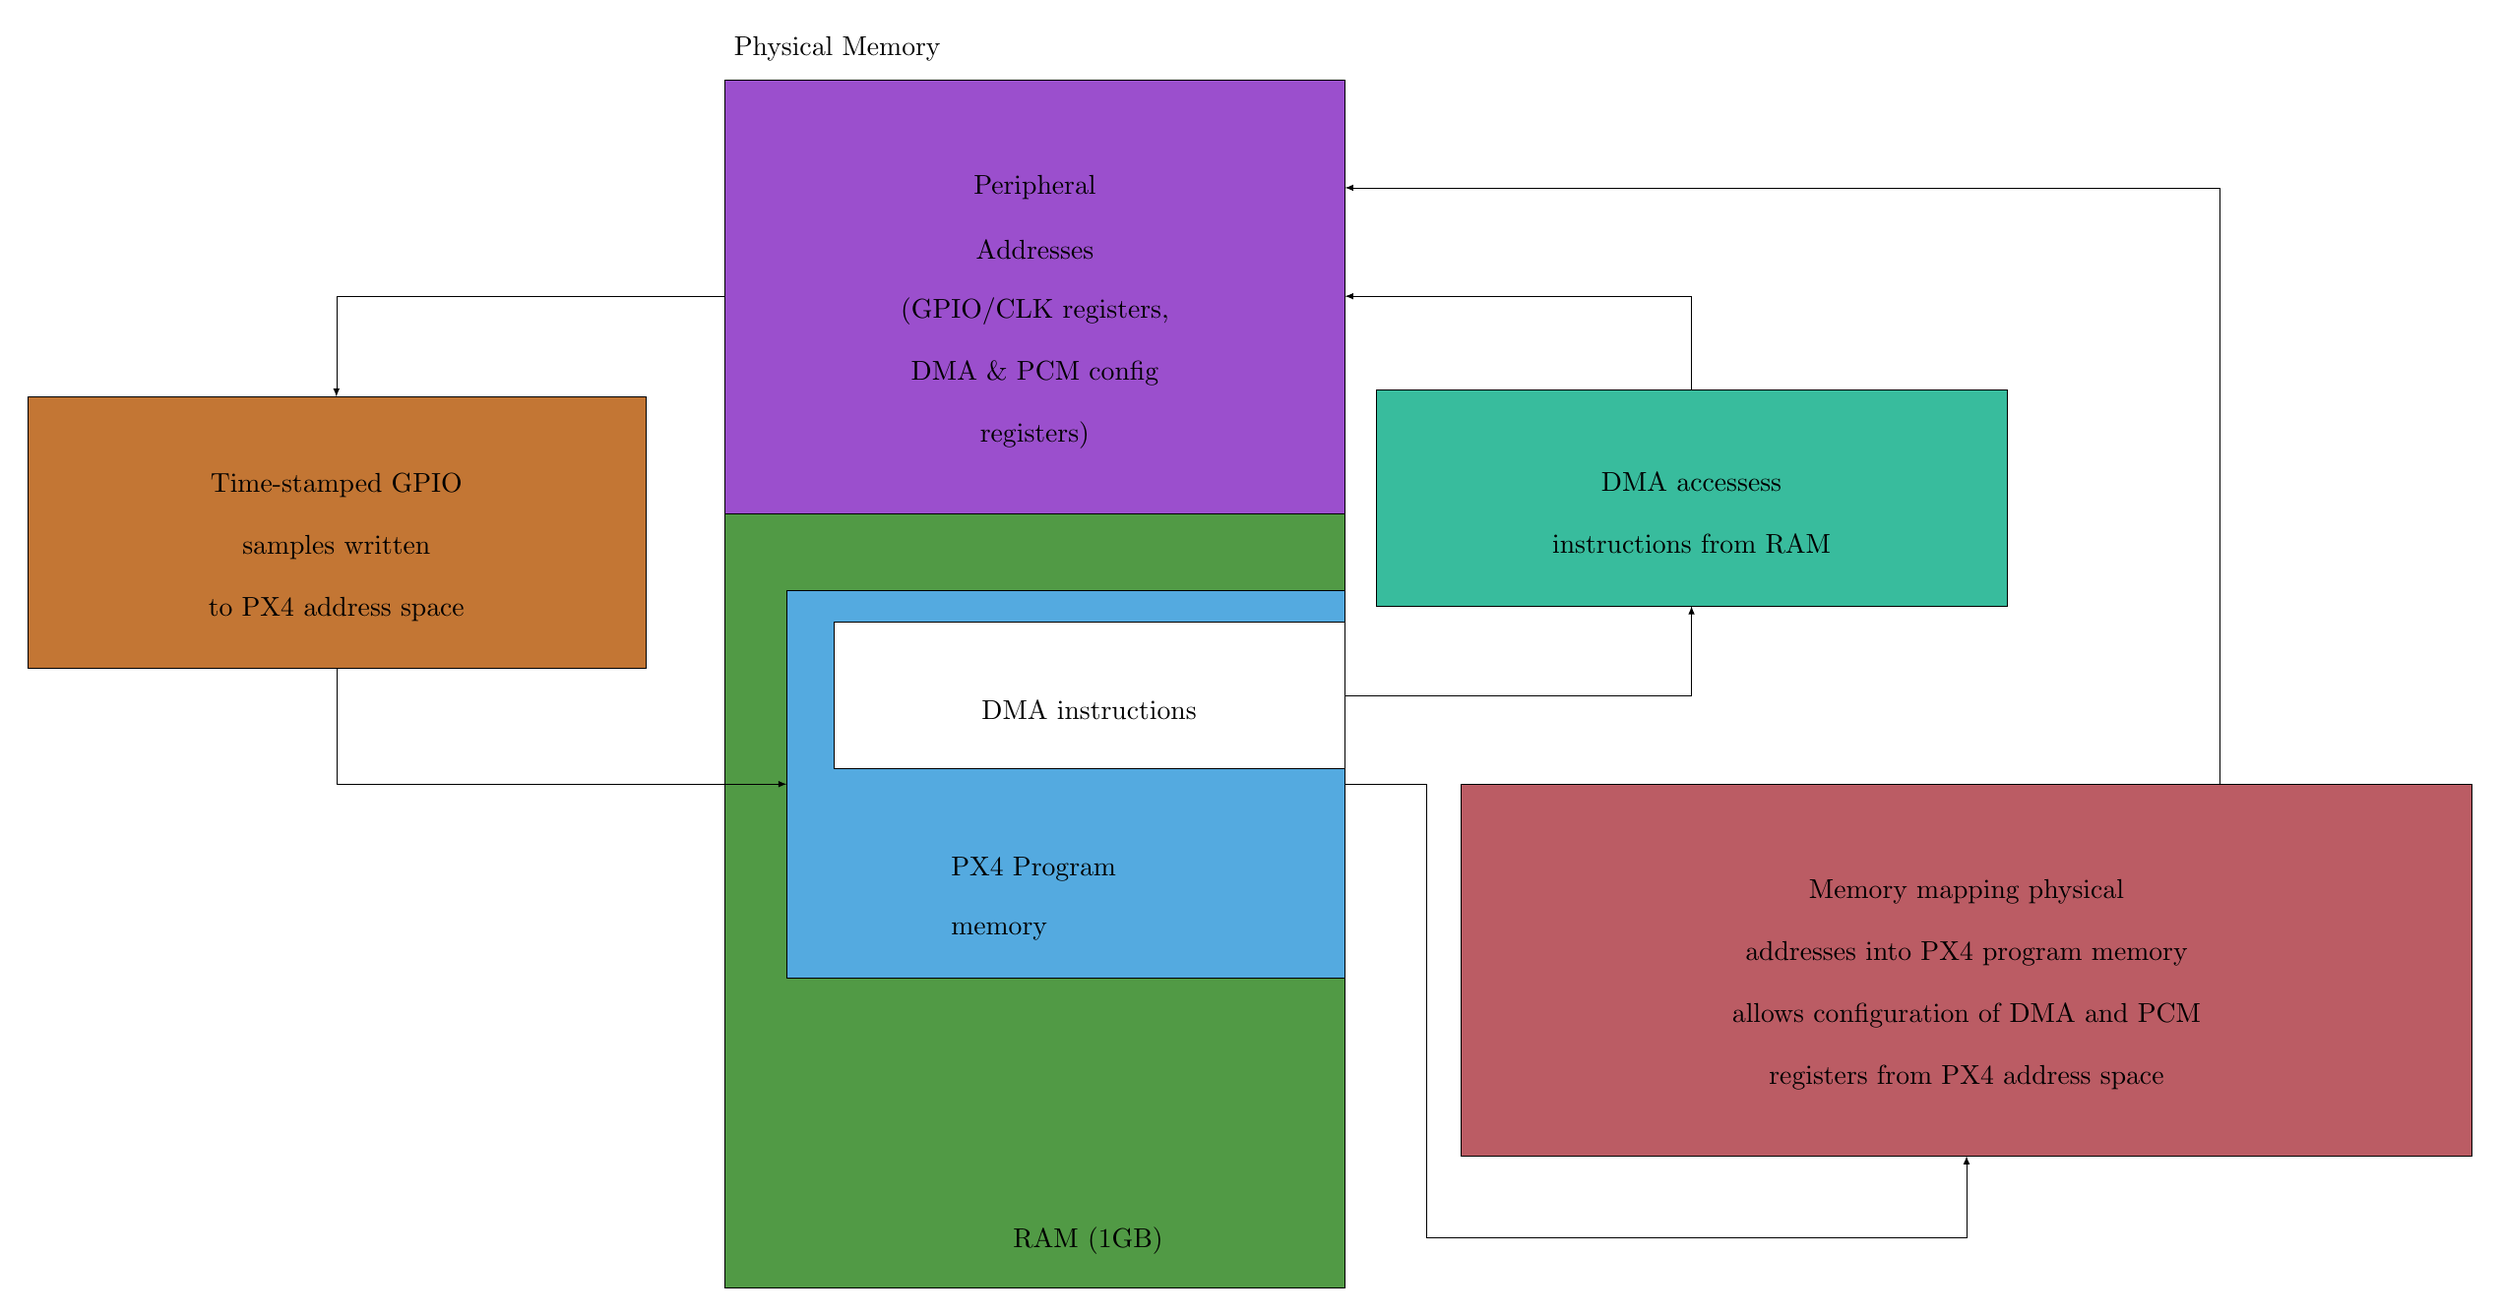
\begin{tikzpicture}
\pgftransformxscale{1.000000}
\pgftransformyscale{-1.000000}
\definecolor{dialinecolor}{rgb}{0.000000, 0.000000, 0.000000}
\pgfsetstrokecolor{dialinecolor}
\definecolor{dialinecolor}{rgb}{1.000000, 1.000000, 1.000000}
\pgfsetfillcolor{dialinecolor}
\definecolor{dialinecolor}{rgb}{0.607843, 0.309804, 0.803922}
\pgfsetfillcolor{dialinecolor}
\fill (7.000000\du,6.400000\du)--(7.000000\du,12.000000\du)--(15.000000\du,12.000000\du)--(15.000000\du,6.400000\du)--cycle;
\pgfsetlinewidth{0.100000\du}
\pgfsetdash{}{0pt}
\pgfsetdash{}{0pt}
\pgfsetmiterjoin
\definecolor{dialinecolor}{rgb}{0.000000, 0.000000, 0.000000}
\pgfsetstrokecolor{dialinecolor}
\draw (7.000000\du,6.400000\du)--(7.000000\du,12.000000\du)--(15.000000\du,12.000000\du)--(15.000000\du,6.400000\du)--cycle;
% setfont left to latex
\definecolor{dialinecolor}{rgb}{0.000000, 0.000000, 0.000000}
\pgfsetstrokecolor{dialinecolor}
\node at (11.000000\du,7.795000\du){Peripheral};
% setfont left to latex
\definecolor{dialinecolor}{rgb}{0.000000, 0.000000, 0.000000}
\pgfsetstrokecolor{dialinecolor}
\node at (11.000000\du,8.595000\du){Addresses};
% setfont left to latex
\definecolor{dialinecolor}{rgb}{0.000000, 0.000000, 0.000000}
\pgfsetstrokecolor{dialinecolor}
\node at (11.000000\du,9.395000\du){(GPIO/CLK registers,};
% setfont left to latex
\definecolor{dialinecolor}{rgb}{0.000000, 0.000000, 0.000000}
\pgfsetstrokecolor{dialinecolor}
\node at (11.000000\du,10.195000\du){DMA \& PCM config};
% setfont left to latex
\definecolor{dialinecolor}{rgb}{0.000000, 0.000000, 0.000000}
\pgfsetstrokecolor{dialinecolor}
\node at (11.000000\du,10.995000\du){registers)};
\definecolor{dialinecolor}{rgb}{0.317647, 0.603922, 0.270588}
\pgfsetfillcolor{dialinecolor}
\fill (7.000000\du,12.000000\du)--(7.000000\du,22.000000\du)--(15.000000\du,22.000000\du)--(15.000000\du,12.000000\du)--cycle;
\pgfsetlinewidth{0.100000\du}
\pgfsetdash{}{0pt}
\pgfsetdash{}{0pt}
\pgfsetmiterjoin
\definecolor{dialinecolor}{rgb}{0.000000, 0.000000, 0.000000}
\pgfsetstrokecolor{dialinecolor}
\draw (7.000000\du,12.000000\du)--(7.000000\du,22.000000\du)--(15.000000\du,22.000000\du)--(15.000000\du,12.000000\du)--cycle;
% setfont left to latex
\definecolor{dialinecolor}{rgb}{0.000000, 0.000000, 0.000000}
\pgfsetstrokecolor{dialinecolor}
\node at (11.000000\du,17.195000\du){};
\definecolor{dialinecolor}{rgb}{0.329412, 0.666667, 0.878431}
\pgfsetfillcolor{dialinecolor}
\fill (7.800000\du,13.000000\du)--(7.800000\du,18.000000\du)--(15.000000\du,18.000000\du)--(15.000000\du,13.000000\du)--cycle;
\pgfsetlinewidth{0.100000\du}
\pgfsetdash{}{0pt}
\pgfsetdash{}{0pt}
\pgfsetmiterjoin
\definecolor{dialinecolor}{rgb}{0.000000, 0.000000, 0.000000}
\pgfsetstrokecolor{dialinecolor}
\draw (7.800000\du,13.000000\du)--(7.800000\du,18.000000\du)--(15.000000\du,18.000000\du)--(15.000000\du,13.000000\du)--cycle;
% setfont left to latex
\definecolor{dialinecolor}{rgb}{0.000000, 0.000000, 0.000000}
\pgfsetstrokecolor{dialinecolor}
\node at (11.400000\du,15.695000\du){};
\definecolor{dialinecolor}{rgb}{1.000000, 1.000000, 1.000000}
\pgfsetfillcolor{dialinecolor}
\fill (8.400000\du,13.400000\du)--(8.400000\du,15.300000\du)--(15.000000\du,15.300000\du)--(15.000000\du,13.400000\du)--cycle;
\pgfsetlinewidth{0.100000\du}
\pgfsetdash{}{0pt}
\pgfsetdash{}{0pt}
\pgfsetmiterjoin
\definecolor{dialinecolor}{rgb}{0.000000, 0.000000, 0.000000}
\pgfsetstrokecolor{dialinecolor}
\draw (8.400000\du,13.400000\du)--(8.400000\du,15.300000\du)--(15.000000\du,15.300000\du)--(15.000000\du,13.400000\du)--cycle;
% setfont left to latex
\definecolor{dialinecolor}{rgb}{0.000000, 0.000000, 0.000000}
\pgfsetstrokecolor{dialinecolor}
\node at (11.700000\du,14.545000\du){DMA instructions};
\definecolor{dialinecolor}{rgb}{0.219608, 0.737255, 0.615686}
\pgfsetfillcolor{dialinecolor}
\fill (15.400000\du,10.400000\du)--(15.400000\du,13.200000\du)--(23.545000\du,13.200000\du)--(23.545000\du,10.400000\du)--cycle;
\pgfsetlinewidth{0.100000\du}
\pgfsetdash{}{0pt}
\pgfsetdash{}{0pt}
\pgfsetmiterjoin
\definecolor{dialinecolor}{rgb}{0.000000, 0.000000, 0.000000}
\pgfsetstrokecolor{dialinecolor}
\draw (15.400000\du,10.400000\du)--(15.400000\du,13.200000\du)--(23.545000\du,13.200000\du)--(23.545000\du,10.400000\du)--cycle;
% setfont left to latex
\definecolor{dialinecolor}{rgb}{0.000000, 0.000000, 0.000000}
\pgfsetstrokecolor{dialinecolor}
\node at (19.472500\du,11.595000\du){DMA accessess};
% setfont left to latex
\definecolor{dialinecolor}{rgb}{0.000000, 0.000000, 0.000000}
\pgfsetstrokecolor{dialinecolor}
\node at (19.472500\du,12.395000\du){instructions from RAM};
\pgfsetlinewidth{0.100000\du}
\pgfsetdash{}{0pt}
\pgfsetdash{}{0pt}
\pgfsetmiterjoin
\pgfsetbuttcap
{
\definecolor{dialinecolor}{rgb}{0.000000, 0.000000, 0.000000}
\pgfsetfillcolor{dialinecolor}
% was here!!!
\pgfsetarrowsend{latex}
{\pgfsetcornersarced{\pgfpoint{0.000000\du}{0.000000\du}}\definecolor{dialinecolor}{rgb}{0.000000, 0.000000, 0.000000}
\pgfsetstrokecolor{dialinecolor}
\draw (15.000000\du,14.350000\du)--(19.472500\du,14.350000\du)--(19.472500\du,13.200000\du);
}}
\pgfsetlinewidth{0.100000\du}
\pgfsetdash{}{0pt}
\pgfsetdash{}{0pt}
\pgfsetmiterjoin
\pgfsetbuttcap
{
\definecolor{dialinecolor}{rgb}{0.000000, 0.000000, 0.000000}
\pgfsetfillcolor{dialinecolor}
% was here!!!
\pgfsetarrowsend{latex}
{\pgfsetcornersarced{\pgfpoint{0.000000\du}{0.000000\du}}\definecolor{dialinecolor}{rgb}{0.000000, 0.000000, 0.000000}
\pgfsetstrokecolor{dialinecolor}
\draw (19.472500\du,10.400000\du)--(19.472500\du,9.200000\du)--(15.000000\du,9.200000\du);
}}
\definecolor{dialinecolor}{rgb}{0.733333, 0.360784, 0.392157}
\pgfsetfillcolor{dialinecolor}
\fill (16.500000\du,15.500000\du)--(16.500000\du,20.300000\du)--(29.542500\du,20.300000\du)--(29.542500\du,15.500000\du)--cycle;
\pgfsetlinewidth{0.100000\du}
\pgfsetdash{}{0pt}
\pgfsetdash{}{0pt}
\pgfsetmiterjoin
\definecolor{dialinecolor}{rgb}{0.000000, 0.000000, 0.000000}
\pgfsetstrokecolor{dialinecolor}
\draw (16.500000\du,15.500000\du)--(16.500000\du,20.300000\du)--(29.542500\du,20.300000\du)--(29.542500\du,15.500000\du)--cycle;
% setfont left to latex
\definecolor{dialinecolor}{rgb}{0.000000, 0.000000, 0.000000}
\pgfsetstrokecolor{dialinecolor}
\node at (23.021250\du,16.895000\du){Memory mapping physical };
% setfont left to latex
\definecolor{dialinecolor}{rgb}{0.000000, 0.000000, 0.000000}
\pgfsetstrokecolor{dialinecolor}
\node at (23.021250\du,17.695000\du){addresses into PX4 program memory};
% setfont left to latex
\definecolor{dialinecolor}{rgb}{0.000000, 0.000000, 0.000000}
\pgfsetstrokecolor{dialinecolor}
\node at (23.021250\du,18.495000\du){allows configuration of DMA and PCM};
% setfont left to latex
\definecolor{dialinecolor}{rgb}{0.000000, 0.000000, 0.000000}
\pgfsetstrokecolor{dialinecolor}
\node at (23.021250\du,19.295000\du){ registers from PX4 address space};
\pgfsetlinewidth{0.100000\du}
\pgfsetdash{}{0pt}
\pgfsetdash{}{0pt}
\pgfsetmiterjoin
\pgfsetbuttcap
{
\definecolor{dialinecolor}{rgb}{0.000000, 0.000000, 0.000000}
\pgfsetfillcolor{dialinecolor}
% was here!!!
\pgfsetarrowsend{latex}
{\pgfsetcornersarced{\pgfpoint{0.000000\du}{0.000000\du}}\definecolor{dialinecolor}{rgb}{0.000000, 0.000000, 0.000000}
\pgfsetstrokecolor{dialinecolor}
\draw (15.000000\du,15.500000\du)--(16.050000\du,15.500000\du)--(16.050000\du,21.350000\du)--(23.021250\du,21.350000\du)--(23.021250\du,20.300000\du);
}}
\pgfsetlinewidth{0.100000\du}
\pgfsetdash{}{0pt}
\pgfsetdash{}{0pt}
\pgfsetmiterjoin
\pgfsetbuttcap
{
\definecolor{dialinecolor}{rgb}{0.000000, 0.000000, 0.000000}
\pgfsetfillcolor{dialinecolor}
% was here!!!
\pgfsetarrowsend{latex}
{\pgfsetcornersarced{\pgfpoint{0.000000\du}{0.000000\du}}\definecolor{dialinecolor}{rgb}{0.000000, 0.000000, 0.000000}
\pgfsetstrokecolor{dialinecolor}
\draw (26.281875\du,15.500000\du)--(26.281875\du,7.800000\du)--(15.000000\du,7.800000\du);
}}
\definecolor{dialinecolor}{rgb}{0.764706, 0.462745, 0.203922}
\pgfsetfillcolor{dialinecolor}
\fill (-2.000000\du,10.500000\du)--(-2.000000\du,14.000000\du)--(5.975000\du,14.000000\du)--(5.975000\du,10.500000\du)--cycle;
\pgfsetlinewidth{0.100000\du}
\pgfsetdash{}{0pt}
\pgfsetdash{}{0pt}
\pgfsetmiterjoin
\definecolor{dialinecolor}{rgb}{0.000000, 0.000000, 0.000000}
\pgfsetstrokecolor{dialinecolor}
\draw (-2.000000\du,10.500000\du)--(-2.000000\du,14.000000\du)--(5.975000\du,14.000000\du)--(5.975000\du,10.500000\du)--cycle;
% setfont left to latex
\definecolor{dialinecolor}{rgb}{0.000000, 0.000000, 0.000000}
\pgfsetstrokecolor{dialinecolor}
\node at (1.987500\du,11.645000\du){Time-stamped GPIO };
% setfont left to latex
\definecolor{dialinecolor}{rgb}{0.000000, 0.000000, 0.000000}
\pgfsetstrokecolor{dialinecolor}
\node at (1.987500\du,12.445000\du){samples written};
% setfont left to latex
\definecolor{dialinecolor}{rgb}{0.000000, 0.000000, 0.000000}
\pgfsetstrokecolor{dialinecolor}
\node at (1.987500\du,13.245000\du){to PX4 address space};
\pgfsetlinewidth{0.100000\du}
\pgfsetdash{}{0pt}
\pgfsetdash{}{0pt}
\pgfsetmiterjoin
\pgfsetbuttcap
{
\definecolor{dialinecolor}{rgb}{0.000000, 0.000000, 0.000000}
\pgfsetfillcolor{dialinecolor}
% was here!!!
\pgfsetarrowsend{latex}
{\pgfsetcornersarced{\pgfpoint{0.000000\du}{0.000000\du}}\definecolor{dialinecolor}{rgb}{0.000000, 0.000000, 0.000000}
\pgfsetstrokecolor{dialinecolor}
\draw (7.000000\du,9.200000\du)--(1.987500\du,9.200000\du)--(1.987500\du,10.500000\du);
}}
\pgfsetlinewidth{0.100000\du}
\pgfsetdash{}{0pt}
\pgfsetdash{}{0pt}
\pgfsetmiterjoin
\pgfsetbuttcap
{
\definecolor{dialinecolor}{rgb}{0.000000, 0.000000, 0.000000}
\pgfsetfillcolor{dialinecolor}
% was here!!!
\pgfsetarrowsend{latex}
{\pgfsetcornersarced{\pgfpoint{0.000000\du}{0.000000\du}}\definecolor{dialinecolor}{rgb}{0.000000, 0.000000, 0.000000}
\pgfsetstrokecolor{dialinecolor}
\draw (1.987500\du,14.000000\du)--(1.987500\du,15.500000\du)--(7.800000\du,15.500000\du);
}}
% setfont left to latex
\definecolor{dialinecolor}{rgb}{0.000000, 0.000000, 0.000000}
\pgfsetstrokecolor{dialinecolor}
\node[anchor=west] at (9.800000\du,16.600000\du){PX4 Program};
% setfont left to latex
\definecolor{dialinecolor}{rgb}{0.000000, 0.000000, 0.000000}
\pgfsetstrokecolor{dialinecolor}
\node[anchor=west] at (9.800000\du,17.400000\du){memory};
% setfont left to latex
\definecolor{dialinecolor}{rgb}{0.000000, 0.000000, 0.000000}
\pgfsetstrokecolor{dialinecolor}
\node[anchor=west] at (10.600000\du,21.400000\du){RAM (1GB)};
% setfont left to latex
\definecolor{dialinecolor}{rgb}{0.000000, 0.000000, 0.000000}
\pgfsetstrokecolor{dialinecolor}
\node[anchor=west] at (7.000000\du,6.000000\du){Physical Memory};
\end{tikzpicture}

        \caption{GPIO sampling memory architecture\label{fig:dma2}}
    \end{figure}

    During development and based on research conducted, we decided not to sample the system clock every second sample, as the timing from the PCM was reliable enough to interpolate. Instead, the clock is sampled once every 14 samples of the GPIO. The selection of this number 14 is explained below. \\

    It is desirable for memory management that both a full loop of DMA control blocks and a full loop of buffer outputs use an integer numbers of memory pages. This requires considering the size of each part of memory we plan to use.

    \begin{itemize}
        \item A page of memory is 4096 bytes under ARMv7 architecture
        \item A DMA control block is 32 bytes
        \item The GPIO register of interest is 4 bytes (32 pins)
        \item The high resolution clock register is 8 bytes
    \end{itemize}

    Taking 14 samples of GPIO and 1 clock sample requires 64 bytes of buffer. We need to do this 64 times to fill out a page of memory. For each 64 byte block of memory used, we require $(14\times2+1) = 29$ DMA instructions. This is because each sample of the GPIO requires one write to the PCM module to reset the sample timer. Since 64 and 29 do not have any obvious common multiples, we resort to reserving 29 pages of memory for the DMA instructions. This gives $29\times 4096 / 32 = 3712$ DMA instructions, which equates to $3712/29/64=2$ pages of timestamped GPIO buffer. So for every 29 pages of DMA instructions, we can get 2 pages of timestamped GPIO data. \\

    It is easy to multiply both sides of this equation out to increase the buffer - for example, we can use $x \times 29$ pages of DMA instructions to get $x \times 2$ pages of GPIO samples. Based on some experimentation, we found that $x=8$ was an appropriate value.\\

    This design was implemented in software under the DriverFramework driver \texttt{ursa\_gpio}. Each of the SONAR and RC drivers were implemented as PX4 modules only, rather than within the DriverFramework. This is because, with the high-speed GPIO sampling issue solved, neither of these modules required any further contact with the hardware. Callback functions were written to allow PX4 methods to be notified of level changes on GPIO pins, and these were used by both the SONAR and RC drivers. \\

    After implementing the GPIO driver module, we found that there were open source alternatives which use a similar design to the one outlined above. In particular, we found a module known as \texttt{PIGPIO}\footnote{\url{http://abyz.co.uk/rpi/pigpio/}}. This module is more comprehensive than our design, since it allows selection of the PWM peripheral for triggering the DMA (as an optional alternative to PCM), and also supports multiple sampling rates for the GPIO. Since this code was freely available under an appropriate license, we ported the relevant sections into our own code base whilst retaining most of our design.

    \subsubsection{Conclusion on sensor interfacing to PX4}
    In order to make our selected sensors work with PX4 and a Raspberry Pi, we were required to use all of the tools at our disposal, as well as apply some creativity to achieve fast GPIO sampling. These methods have been successful. We were able to confirm that data from our sensors were available to other components within the PX4 ecosystem (such as the controller). We were also able to confirm that PX4 was capable of writing to our hardware (for example, writing commands to the PWM chip for output).

\section{Handheld Mapping}

After interfacing the drone with sensors, the next step is to construct a map while the drone is in a stationary position.   The goal is to send laser scans via WIFI to the ground-station where the data is interpreted by SLAM software.  Achieving this requires the completion of a series of intermediate steps:

\begin{itemize}
    \item Receive laser scan data (from one machine)
    \item Communicate with the drone via ground- station
    \item Visualize laser scanner data
    \item Interpret scans to estimate position within a map
    \item Clean laser scan data
\end{itemize}

\subsection{Receiving Laser Scan Data}
We begin by discussing the communication of laser scan data between the drone and desktop.  In section XXXX ROS was selected as the middleware to enable communications across systems.   Some of the benefits of using ROS were also discussed, namely it’s package-based ecosystem making thousands of robotics and automation software available for use.  In this section we discuss ROS in more depth.  We cover the main components of ROS, it’s guiding principles and how they were used to communicate laser scan data between devices.\\

As mentioned previously packages are the primary organisation unit within ROS.  Packages are written to address a specific problem such as communicating laser scanner data or computing mathematical transfers.  They can simply be thought of as a folder containing a number of scripts, executable and other artefacts. The definition of a package is kept intentionally minimal by ROS to support their guiding philosophy of being ‘thin’\footnote{See http://www.willowgarage.com/sites/default/files/icraoss09-ROS.pdf}.  Therefore the only required components are an XML package description and a CMakeLists.txt file for the build system.  To test our communication link we wrote our own ‘debug’ package. Creating a package can either be done manually or via the utility command:

\begin{lstlisting}[language=bash]
    catkin_create_package <package name> <dependency 1> <dependency 2> ... 
\end{lstlisting}

 Figure \ref{fig:package_xml} shows an example of the XML script required to define our package.  Note that only a few fields are required with the most important being the package name. Given a package exists for communicating laser scan data, it may seem unnecessary to write our own package.  However to enable communication between drone and desktop, additional commands need to be called rather than just initialising the laser node.  These could be called sequentially through the command line but would need to be re-typed each time.  A package is a more elegant solution and allows the inclusion of a number of other debugging scripts.

 \begin{figure}[H]
    \begin{lstlisting}[language=xml]
        <name>debug</name>
        <version>1.0.0</version>
        <description>Debugging scripts</description>
        <maintainer email="ihook@student.unimelb.edu.au">Isaac Hook</maintainer>
        <license>BSD</license>
    \end{lstlisting}
    \caption{Package.xml file required to define a package}\label{fig:package_xml}
\end{figure}

Whereas a package is the software organisation unit of ROS, a node is the primary computational unit.  A node can just be thought of as an executable that uses ROS to communicate with other nodes.  The simplest "computation graph" may be one node continually printing "hello world" and another node listening to the output (included in URSA debug).  Of course nodes can perform any desired computational task, for example: filtering laser scan data, calculating costs associated with navigating an environment or printing the height data for an ultrasonic component.  In our case we want to interface the Hokuyo UG01 with our drone.  As detailed in section XXXX we search the ROS documentation and find that the "urg\_node" package works with any SCIP 2.2 or earlier laser range finders.  An alternative method of installing a package if access to the source code is not required is simply$...$

\begin{lstlisting}[language=xml]
    sudo apt-get install ros-kinetic-urg-node
\end{lstlisting}

After installing the required node we can utilise the ROS command line interface to explore the package.  For example we can query the installation location with teh following command:

\begin{lstlisting}[language=xml]
    rospack find urg_node -> /opt/ros/kinetic/share/urg_node
\end{lstlisting}

Using tab completion we can see a list of all nodes in the urg\_node package.  We can see it is a small package only containing a few nodes.

\begin{lstlisting}[language=xml]
    rosrun urg_node <TAB> <TAB> -> getId urg_node set_urg_node_ip.py
\end{lstlisting}

These nodes directly line up with our explanation of them as executables.  Figure \ref{fig:executable} shows the CMakeLists.txt file defining the C++ executables.  In addition the python script “set\_urg\_ip.py” appears as it does not need to be compiled.

\begin{figure}[H]
    \begin{lstlisting}[language=c++]
    ## Declare a cpp executable
    add_executable(urg_node src/urg_node.cpp)
    target_link_libraries(urg_node urg_node_driver ${catkin_LIBRARIES})

    ## Declare getID tool
    add_executable(getID src/getID.cpp)
    target_link_libraries(getID urg_c_wrapper ${catkin_LIBRARIES})
    \end{lstlisting}
    \caption{Executable definitions in CMakeLists.txt}
    \label{fig:executable}
\end{figure}

Our current understanding of ROS is that of a peer-to-peer computational graph, however we haven't discussed how nodes talk to each other.  To enable communication between these nodes, named buses called topics are used.  Topics are identified simply by strings.  For example a topic receiving laser scan data may be called "/scan".  Topics place few restrictions on their use by nodes.  A node wanting to receive data from a particular topic can subscribe to it.  A node wanting to send data to a particular topic may publish to it.  Multiple nodes can subscribe to one topic.  Similarly multiple nodes can publish to one topic.  A node publishing or subscribing to a topic is not aware of the node on the other end.  In this way the production and consumption of information is independent.   One important restriction placed on topics is that only one message type can be communicated over it.\\

Nodes communicate with other nodes by publishing messages to topics.
A message is defined by nothing more than a multi-line text file.  One column specifies data type while the other sets the names.  As with other features of ROS, messages are kept intentionally thin.  Text files are language neutral and therefore support cross-language development, which is another guiding principle of ROS.  Primitive data types such as float, int, string and array are allowed.  In addition, a message itself can be defined as a data type allowing unlimited nesting.  In this section we are primarily concerned with sending messages containing laser scan data.  A laser scan message is a common type in robotics and as such there is an existing definition used by package developers\footnote{http://docs.ros.org/api/sensor\_msgs/html/msg/LaserScan.html}.  This message type is used by the urg\_node (Figure \ref{fig:message}).  Note that the majority of the fields are primitive types (float32 or float32[]).  "Header" is an example of a nested message type, which is commonly used to uniquely identify and timestamp data.

\begin{figure}[H]
    \begin{lstlisting}[language=c++]
        std_msgs/Header header      # field timestamps data from first ray in scan
        float32 angle_min           # start angle of scan
        float32 angle_max           # end angle of scan
        float32 angle_increment     # distance between measurements
        float32 time_increment      # time between measurements 
        float32 scan_time           # time between scans
        float32 range_min           # minimum range values
        float32 range_max           # maximum range value
        float32[] ranges            # array containing ranges
        float32[] intensities       # some laser scanners support intensity readings
    \end{lstlisting}
    \caption{Message definition file of LaserScan.msg}
    \label{fig:message}
\end{figure}

Having discussed the concepts of packages, nodes, topics, message;
getting the laser data scanner streaming on one machine is now straightforward.  After setting up the correct USB permissions, the following commands must be run.

\begin{lstlisting}[language=bash]
    Roscore
    Rosrun urg_node urg_node
\end{lstlisting}

Roscore is a command to start a collection of nodes and programs that are required to run a ROS based system.  The main components that are started are 
\begin{itemize}
    \item ROS master
    \item Parameter server
    \item Rosout logging node
\end{itemize}

The ROS master is essentially a name sever that enables nodes to communicate with each other.  Without the master, nodes would not be able to find each other in the network.  The parameter server can be thought of as a list of variables and their values accessible by any node.  The logging node provides console log output.  Rosrun starts the executable ‘urg\_node’ located in the package ‘urg\_node’.\\

The node ‘urg\_node’ is now running.  We can use a number of utility commands to confirm is system is behaving as expected.  "rosnode list" shows that only the nodes \/rosout (from roscore) and \/urg\_node are running.  Similarly "rostopic list" shows topics associated with rosout have been created and also our topic "/scan" used to publish scan data to.  "rostopic type /scan" confirms that the message type of the topic /scan is in fact sensor\_msgs/LaserScan as stated above.

\begin{lstlisting}[language=bash]
    rosnode list        -> /rosout /urg_node
    rostopic list       -> /rosout / rosout_agg /scan + others
    rostopic type /scan -> sensor_msgs/LaserScan 
\end{lstlisting}

To see the output of our laser scan data we type "rostopic echo /scan".  Figure \ref{fig:laser_snippet} shows a snippet of the raw data.  We can see that the data adheres to the typed definitions named in the .msg file.

\begin{figure}[H]
    \centering
\begin{lstlisting}[language=c++]
        header: 
          seq: 4195
          stamp: 
            secs: 1506932516
            nsecs: 774564046
          frame_id: laser
        angle_min: -2.35619449615
        angle_max: 2.09234976768
        angle_increment: 0.00613592332229
        time_increment: 9.76562732831e-05
        scan_time: 0.10000000149
        range_min: 0.019999999553
        range_max: 5.59999990463
        ranges: [0.01899999938905239, 0.01899999938905239, ...
    \end{lstlisting}
    \caption{Snippet of laser scan data}
    \label{fig:laser_snippet}
\end{figure}

\subsection{Communicate with the drone via ground-station}
One philosophical goal of ROS is that it is a peer-to-peer network across of distributed hardware connected at runtime.  This design principle allows for any number of nodes to communicate with each other across multiple machines.  As a result, receiving laser scan data generated on one system (drone) on another system (ground-station) is simplified under the ROS framework.\\

The basic requirements are to have bi-directional connectivity on all ports, one master and all using same ROS master URI.  To establish a network, the Raspberry Pi was set up as an access point to which the ground-station was connected.  ROS\_MASTER\_URI is a Linux environment variable setup after the installation of ROS.  It can be altered directly in the terminal by setting the variable to the desired value.  In our case it makes sense to use the ground-station as the master, therefore we set this variable on the Raspberry Pi to be equal to the address of the ground-station.

\begin{lstlisting}[language=bash]
    export ROS_MASTER_URI = http://<hostname_of_groundstation>:11311
\end{lstlisting}

Under this setup we can now receive laser data on the ground-station.  However even for this simple scheme the number of commands required can become cumbersome.  By way of example the commands needed are given below (assuming code has been compiled).

\begin{lstlisting}[language=bash]
    # ground-station
    Rocore 
    Rostopic echo /scan

    # Raspberry Pi from groundstation
    ssh pi@<hostname_of_pi>
    cd catkin_ws
    source devel/setup.bash
    roscore
    rosrun urg_node urg_node
\end{lstlisting}

Although this number of commands may seem somewhat tractable, this is a relatively simple example.  As more capability is added to the system, multiple nodes will need to be initiated.  For example - one node to publish laser scanner data, another to publish ultrasonic data, nodes for navigation and visualization.  Having to manually type \texttt{rosrun <package name> <node>} will undoubtedly slow down development time and is prone to errors.  A natural solution to this problem would be to suggest the creation of a node to handle the running of all other nodes, after all a node is just an executable.  This would be possible, python for instance has the "os" and "subprocess" library which both allow the execution of terminal commands.  Python scripts could be run on the master that ssh to the Pi and run terminal commands. However, there is a better solution developed by ROS specifically for this application, launch files.\\

Launch files are XML files that can be configured to run multiple nodes distributed across machines.  The benefit of using launch files is that, given ROS is setup correctly, configuring a node to run is a one line XML tag.  In addition to running nodes, topics can be renamed for one node.  Renaming topics is useful if different manufactures/developers use different topic names to communicate the same data.  Although we haven’t discussed the parameter server in depth, these values can also be set from a launch file. Re-spawning nodes that have died and choosing which machine to run can be achieved easily be specifying simple XML arguments.\\

In our case we need to write a launch file that launches the urg\_node on the Raspberry Pi and the \texttt{rostopic echo} command on the desktop.  Ideally we would like to be able to run this just from the ground-station.  Figure \ref{fig:launch_file} shows the launch file written to achieve this.  To stream laser scan data to the ground-station now requires only the execution of one command: 

\begin{lstlisting}[language=bash]
    roslaunch debug laser_debug.launch
\end{lstlisting}

\begin{figure}[H]
    \centering
    \begin{lstlisting}[language=xml]
    <launch>
    <!-- Setup urg_node -->
    <machine name="drone" address="10.42.0.101" user="pi"/>
    <node machine="drone" name="urg_node" pkg="urg_node" type="urg_node" 
          respawn="true"/>

    <!-- Echo scan data -->
    <node name="echo_scans" pkg="rostopic" type="rostopic" args="echo \scan" 
          respawn="true" output="screen"/>

    <!-- Load robot description file to paramter server -->
    <param name="robot_description" textfile="$(find debug)/urdf/ursa.urdf"/>

    <!-- Use robot description to publish /tf node -->
    <node name="robot_state_publisher" pkg="robot_state_publisher" 
          type="robot_state_publisher"/>
    </launch>
    \end{lstlisting}
    \caption{Launch file to receive laser scanner produced by drone on ground-station}
    \label{fig:launch_file}
\end{figure}

In summary, ROS can be thought of a computation graph made up of nodes.  Nodes communicate with other nodes by publishing messages to topics and receive data by subscribing to topics.  To send laser scan data to the desktop we installed the urg\_node on the Raspberry Pi.   To print laser scan data to the screen we created an echo node on the desktop.  Figure \ref{fig:ROS} captures these high level concepts graphically.

\begin{figure}[H]
    \centering
    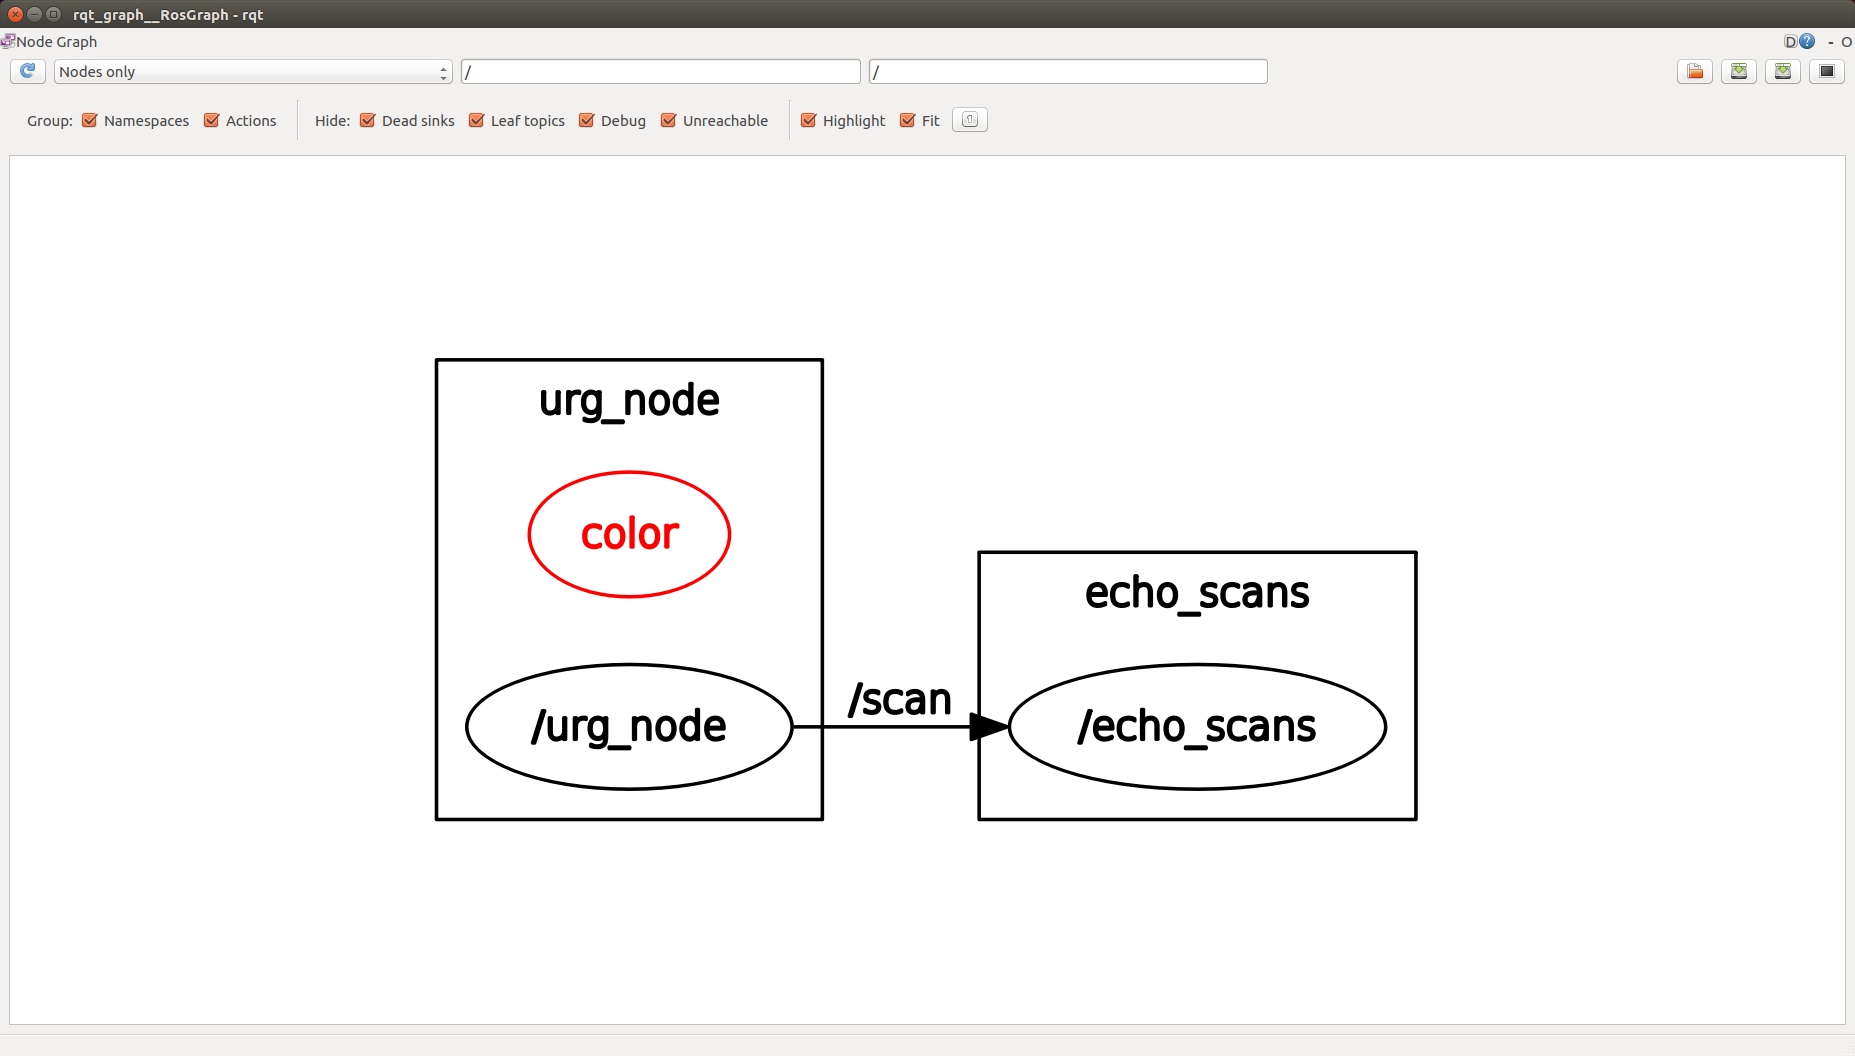
\includegraphics[width=0.8\linewidth]{imgs/node_graph.png}
    \caption{ROS nodes, topics and messages}
    \label{fig:ROS}
\end{figure}

\subsection{Visualize laser scanner data}

As shown in Figures \ref{fig:message} and \ref{fig:laser_snippet}, laser scanner data is primarily composed of range measurements updated at \SI{10}{\hertz}.  Values such as minimum angle and angle increment are given so that all laser points can be derived relatively from the first point.  In it’s raw form it is difficult to interpret the data and confirm that readings received are in fact giving measurements representative of the surroundings.  Therefore the next step to be taken is to visualize the range data.\\

It would not be difficult to write a custom solution using python for instance.  However, ROS already has it’s own visualization tool which natively can subscribe to topics and plot a particular data type.  RVIZ\footnote{http://wiki.ros.org/rviz} recognizes important message types such as laser scans, point clouds, geometric primitives and poses out of the box.  This capability reinforces the usefulness of ROS.  Multiple sources of data may communicate using the same message type for example a navigational goal and current robot pose may both use a pose message type.  Naming and colouring of the received data can then be done in RVIZ based on the topic name.  Therefore the visualization of data is decoupled from the generation of data.  In addition, plugins can be written to display more types of data.  We utilise this feature in section XXXX where a module is written to subscribe to camera data.\\

Laser scans adhering to the sensor\_msgs/Laser\_scan type are supported by RVIZ.  By running our previous launch script and executing the command \texttt{rosrun rviz rviz} we can effortlessly visualize the point cloud.  Figure \ref{fig:RVIZ_laser} shows the output.

\begin{figure}[H]
    \centering
    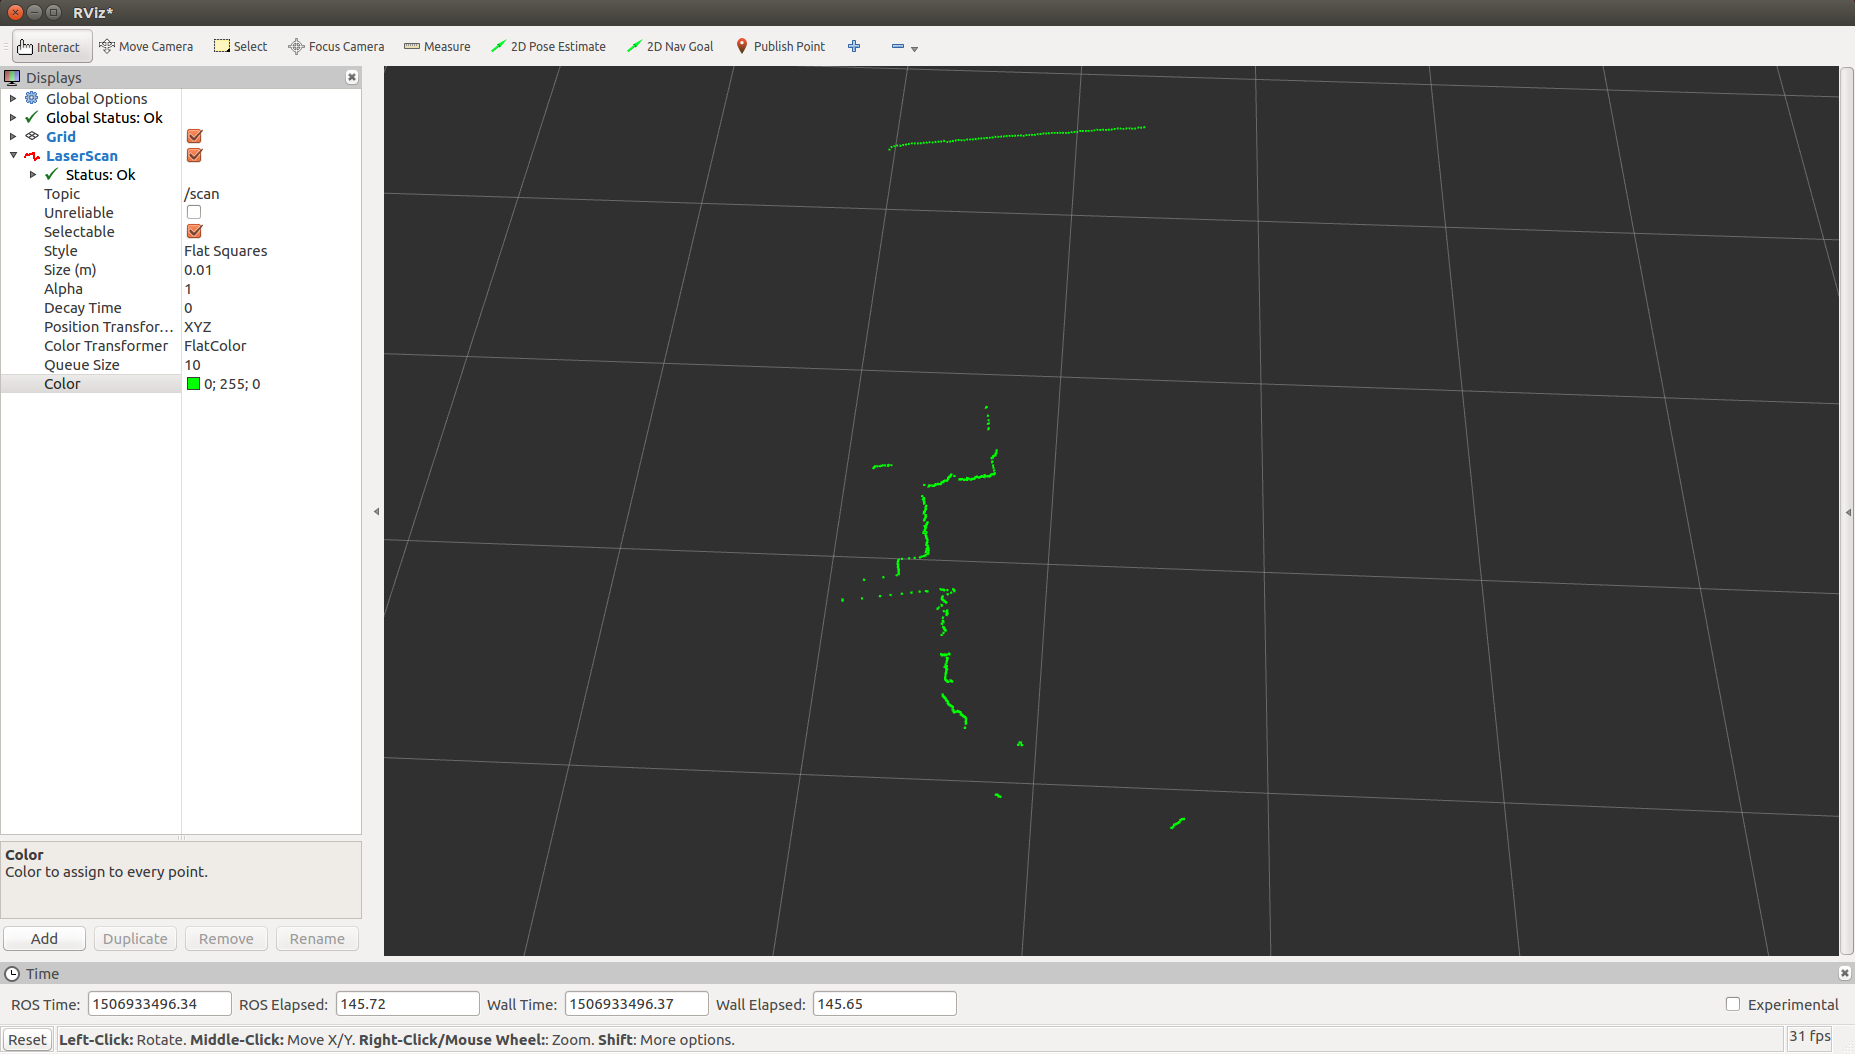
\includegraphics[width=0.8\linewidth]{imgs/laser_scan_rviz.png}
    \caption{Visualization of laser scan data}
    \label{fig:RVIZ_laser}
\end{figure}

\subsection{Cartographer}
At this stage we have successfully communicated laser scan data generated by the drone to the ground-station.  Data has been visualized as a point cloud in RVIZ.  However, just by generating this data does not mean that the drone is able to locate itself within the environment.  The next step is to implement a SLAM algorithm as discussed in previous sections that is able to interpret the data and provide the drone with an estimate of its position.

\subsection{Filtering Laser Scan Data}


\section{Project milestone - Hovering in place}
Having developed sensor interfaces, as well as having tested our SLAM solution in simulation, we were within striking distance of the first milestone of the URSA prototype. This consists of having the UAV takeoff, hold position in a room using LiDAR scan data for an arbitrary amount of time, and then land. If this can be achieved, we will have demonstrated that our combination of LiDAR scans and offboard Cartographer will have successfully replaced the GPS used in conventional outdoor UAVs. This could then be extended to obstacle avoidance and pathfinding, also using the output of Cartographer.\\

In order to achieve this first project milestone, the following system components needed to be developed and improved:
\begin{itemize}
	\item Providing power to the prototype system
	\item Fusion of the position estimate provided by Cartographer into the EKF used by PX4
	\item Development of a basic user interface for instigation of take-off and landing. In the future, this interface will also provide more advanced navigation and configuration options.
\end{itemize}

Each of these components is discussed below.

\subsection{Power}
Prior to prototype testing, we were able to provide power to the Raspberry Pi via a USB cable from a wall outlet. In an actual flight, the motors also require power, and the ESCs are designed to operate off around \SI{12}{\volt}. The Erle-Copter also includes a buck converter which provides \SI{5}{\volt} power to the Pi from the same \SI{12}{\volt} rail.\\

One solution could be to use the battery provided with the Erle-Copter. However, this battery can only provide around 20 minutes of continuous flight time, after which it requires around 8 hours to charge. This is not acceptable in a rapid development environment. We therefore decided to provide a tethered source of \SI{12}{\volt} power.\\

Our first solution was to use a small \SI{12}{\volt} AC to DC regulator which had previously been used in the laboratory for powering UAV flight. However, on attempting to take-off using this supply, the motors could not generate enough thrust to lift URSA off the ground. On inspection of the power supply, we found a maximum current rating of \SI{10}{\ampere}. The ESCs on URSA are rated to \SI{30}{\ampere} each, for a total possible current consumption of \SI{120}{\ampere}. Clearly, the first power supply tested was insufficient. \\

We then moved onto a desktop power supply, rated at \SI{600}{\watt}, allowing \SI{50}{\ampere} current output on its \SI{12}{\volt} rail. This power supply is designed for very high power consumption desktop components, such as graphics cards and high-end CPUs. We found that this power supply provided sufficient current to allow take-off when the LiDAR scanner was not attached, but not with the LiDAR scanner attached.\\

Our first instinct was to simply increase the power supply capacity again. However, on reflection, it was not possible that URSA would require \SI{50}{\ampere} to simply take off and hover, even with around \SI{100}{\gram} load. This can be checked by noting that the provided \SI{5000}{\milli\ampere\hour} battery provides an apparent flight time of 20 minutes. This means expected current consumption should be around \SI{15}{\ampere} for hovering. It's unlikely that adding a small weight would increase this to \SI{50}{\ampere}. It is also nowhere near the current capacity of the motors - as mentioned above, this limit is around \SI{120}{\ampere}.\\

The solution was to measure the voltage at the regulator and compare it to the voltage seen onboard the UAV. We found that this was, as expected, \SI{12}{\volt} when the motors weren't running; however it sagged to around \SI{8}{\volt} on the UAV when the motors started running. The voltage at the regulator was still \SI{12}{\volt}, even with the motors running. This tells us that the regulator is under no stress when providing the output current, and the problem is in the voltage drop over our cable to the drone. \\

The cable we were using was approximately \SI{4}{\meter} long, advertised for high current, low voltage applications, manufactured by OLEX. Inspecting the conductor dimensions, we found that it was \SI{2.5}{\milli\metre\squared}. This equates to around 13AWG. While we couldn't find the exact cable on the suppliers website, a similar cable\footnote{\url{http://www.olex.com.au/eservice/Australia-en_AU/navigateproduct_540307840/CACP07A1002WVAA.html\#characteristics}} was advertised as having a maximum DC resistance of \SI{7.41}{\ohm\per\kilo\metre}. This gives us a total resistance of \SI{0.059}{\ohm}, including the return path. The voltage drop is therefore expected to be up to \SI{3}{\volt} for the maximum DC output of our power supply.\\

The reason why we appeared to be experiencing slightly more than the \SI{3}{\volt} drop is unclear, but one possible explanation may be the quality of the terminal connections, which introduce additional resistance. Another explanation may be that we only tested the voltage drop via a multimeter, which typically integrates its measurement over short time periods. If there are large spikes in current, this may cause the multimeter to report a lower average voltage than what might be expected from simply looking at average power delivered to the motors. \\

Regardless of this minor variance, it is clear that the cabling to power our motors was not sufficient. The problem was easily resolved by replacing the cable with a shorter 8AWG equivalent. This new cable has a resistance approximately $\frac{1}{3}$ the value of a 13AWG cable per unit distance. Using this cable, the voltage drop was reduced to around \SI{1}{volt}, and the prototype was able to lift off with the LiDAR load.

\subsection{EKF Fusion}
The next challenge in achieving stable flight was to feed Cartographer localization information back through the PX4 estimation algorithm. It was straightforward to provide this data over MAVROS using techniques already discussed. Cartographer generates a 2D transform from the origin to the UAV. We wrote a script, \texttt{height\_publisher.py}, which consumes this transform and publishes a new 3D transform which accounts for the data received in the SONAR height sensor. This was then sent to PX4 via the \texttt{vision\_pose\_estimate} topic within MAVROS. 

The \texttt{vision\_pose\_estimate} topic is designed to send a position and orientation which has been computed by an offboard system. Fusing this data with existing sensors onboard the UAV was slightly more involved and required modifications to the state estimation algorithms within PX4. \\

The default algorithm for state estimation used by PX4 is known as the `local position estimator' (LPE) in conjunction with an attitude estimator. However, this design is in the process of being replaced by a superior EKF which jointly estimates both position and attitude. There are 24 states in the EKF model, and their relationship for the predict/correct EKF equations has been derived symbolically via MATLAB script \footnote{See \url{https://github.com/PX4/ecl/blob/master/matlab/scripts/Inertial\%20Nav\%20EKF/GenerateNavFilterEquations.m}}.\\

The advantage of the EKF over the simpler LPE algorithm is that it supports a so called `delayed fusion time horizon'. This allows the fusion of multiple observation sources which may only be available after a delayed time. This is very useful for GPS data, but can also be re-used for our purposes with Cartographer data. The advantage of either algorithm over a simple averaging filter or using Cartographer data directly is it allows much faster responses to changes in position or attitude, as detected by the IMU onboard URSA. \\

However, the drawback to the EKF used in PX4 is that it is in an experimental state. In particular, the aspect of the system which we propose to use (vision position fusion) is not very well tested. For example, we found that there were overrides when using vision position fusion but not GPS data. This was preventing PX4 generating estimated pose outputs. This is obviously a poor design, as it does not account for cases where `vision estimates' are used in place of GPS.\\

To resolve these issues, we first compiled PX4 to use the experimental EKF instead of the default LPE. We then attempted to configure this environment to work in simulation. We found that some code changes to the EKF were required, and created our own fork of this library. In debugging the code, we found that there were a number of bugs which weren't specific to URSA, but the EKF library generally. In the spirit of open source code, we made our improvements available back to the PX4 team\footnote{\url{For example see https://github.com/PX4/ecl/issues/296}}. \\

Eventually, we were able to get the vision position estimation working as required within the EKF. This allowed us to conduct flight tests in simulation.

\subsection{Interface for taking off}
The final aspect of achieving the first milestone was being able to instruct URSA to take-off to a certain height, and to land. Our long-term solution to this was to design and develop a user interface which could be implemented as a panel within RVIZ. However, for initial testing, we developed a simple terminal application which took text inputs. \\

This application was built as a python script, \texttt{controller.py}. This script eventually evolved into a program which managed all input and instructions to URSA, including navigation events. However, the first version simply allowed take-off by arming the drone and providing a set-point. Landing was accomplished by putting a set-point on the ground, and then disarming after a constant time.\\

Testing was extremely positive and showed that the drone was able to take off and hold position. Even when pulled away from the set-point, the drone would return to the same spot. Videos of the tests undertaken for this first milestone are available at \url{https://youtu.be/w-l4K_zTDDQ} and \url{
https://youtu.be/xKCTSxtxNYs}.\\

Having achieved this first milestone, we then move onto the design of obstacle avoidance and navigation algorithms, which occupied us for the remainder of the capstone project.

\section{Navigation}

At this stage we have now successfully integrated sensor data to simultaneously estimate the drones position and build a map.  We have also completed an initial test flight with the drone hovering to a set height and landing.  As mentioned in the scope of the project our main goal is to develop a drone that can navigate an indoor test environment whilst achieving the following:

\begin{itemize}
    \item Mapping stationary obstacles
    \item Avoid both stationary and non-stationary obstacles
    \item Be able to navigate to a set point uploaded by operator
\end{itemize}


To achieve these goals we once again turn to ROS.  The navigation stack is a package that offers 2D navigation.  We restrict our navigational capabilities to 2D as we are using a planar laser for our primary position estimation tool.  A planar laser could be used for 3D navigation, the PR2 robot used by Eitan et. al produced 3D scans by tilting the laser \footnote{http://wiki.ros.org/Papers/ICRA2010\_Marder-Eppstein}.  On a drone platform the height could be adjusted to get multiple 2D slices of the environement.  However we considered 3D scans as out of scope and an area for expansion. \\

At a high level the navigation stack can be thought of as a black box accepting sensory information (laser scans, odometry readings, height) and a target pose.  As output the package sends velocity commands to a mobile base.  The navigation stack is composed of several main components.  We introduce the high-level concepts here before discussing them in more depth.  At the heart of the navigation stack are trajectory planners and costmaps.  Trajectory planners take the current robot position and some goal and generate potential paths.  The costmaps influence the selection of optimal path by ensuring that trajectories do not pass through or too close to obstacles.  Both the trajectory planners and costmaps have local and global versions.\\

The global planner takes inputs from the global costmap, goal setpoint and generates the best long term plan.  The local planner considers the local costmap, current laser scan information and position to find the best path along the global plan.  A primary goal of the local plan is to ensure that it avoids obstacles whilst advancing towards the local goal.  In some instances the robot may get stuck.  The navigation stack handles these occurrences by initiating recovery behaviours.\\

Each of these components can be developed separately as long as they adhere to the interface specified in the navcore package.  The move base package connects them together to achieve a global navigation task.\\

Figure \ref{fig:nav_stack} shows our setup and summarises the high-level concepts of the navigation stack.  The XXXX coloured boxes highlight the components, which were modified by URSA.  In the following subsections we cover the components of the navigation stack in more detail.  We dedicate more focus to those that were modified/added by URSA.

\begin{figure}[H]
    \centering
    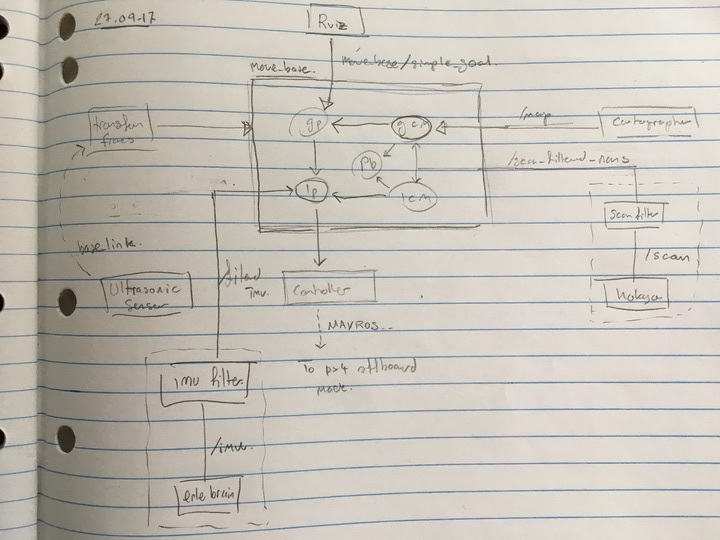
\includegraphics[width=0.7\textwidth]{imgs/nav_stack.jpg}
    \caption{Core components of the navigation stack\label{fig:nav_stack}}
\end{figure}

\subsection{Global Planner \& Costmap}

No changes were needed to be made to the global planner and global costmap.  The team were only faced with the choice of global planner.  There are three main global planners offered by ROS; carrot, global\_planner and navfn.\\

The carrot planner is the simplest of the three and works by drawing a straight line between robot and target.  If the goal point is an obstacle the carrot planner moves the point closer to the robot until it is no longer over an obstacle.  This type of planner has obvious limitations.  For example a desired capability of the global planner is to be able to place a goal in an unexplored environment.  If an obstacle such as a corner obstructs a desired setpoint the planner wont be able to resolve a valid path.  This is obviously not optimal behaviour as a corner should be navigable.  Even in explored space such a planner would be cumbersome to use as valid paths would have to be identified by the human operator and constructed using straight line segments.

\begin{figure}[H]
    \centering
    \begin{subfigure}{.5\textwidth}
        \centering
        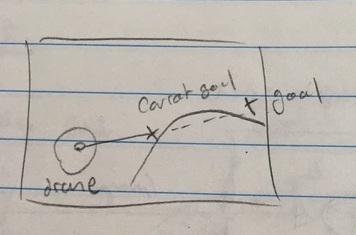
\includegraphics[width=0.7\textwidth]{imgs/carrot_planner_a.jpg}
        \caption{Navigating a corner}
    \end{subfigure}%
    \begin{subfigure}{.5\textwidth}
        \centering
        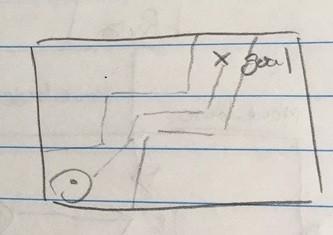
\includegraphics[width=0.7\textwidth]{imgs/carrot_planner_b.jpg}
        \caption{Path to be drawn by operator}
    \end{subfigure}
    \caption{Carrot planner\label{fig:carrot}}
\end{figure}

We opted to use the default global planner, navfn, that comes with the move base package. The navfn package works by implementing Dijkstra’s algorithm on the costmap cells to find the optimal path\footnote{http://wiki.ros.org/navfn}.  Dijkstra’s algorithm is a common “shortest-path algorithm” for weighted graph problems.   Unlike the carrot planner, paths avoiding obstacles can be generated because of the formulation of the problem as a graph.  Simulation showed that this planner was sufficient for our purposes.\\

The main difference between the global\_planner implementation and navfn is that an optimised A* algorithm is available in the global\_planner\footnote{http://wiki.ros.org/global\_planner}.  The A* algorithm is more efficient by employing the use of heuristics.  However, Dijkstra’s algorithm will find the optimal path because it employs breadth first search (considers all points).\\

Having chosen a global planner, the purpose of a local planner may not be immediately obvious.  If we are generating a global costmap and the global path respects these limitations, why not just follow the global plan?  One important reason is the distinction between the local and global costmap.  The global costmap is constructed from a static map whereas the local costmap is created real time sensor data.  Therefore any moving obstacles or uncertain areas in the map will not be accounted for in the global plan.  The global planner does not take into account the dynamics of the robot and makes assumptions (e.g. circular robot) to ensure efficiency of the planning algorithm.  As a result the global path may produce a target trajectory that is overly optimistic such as rounding a corner too sharply or selecting a plan through a gap that is too narrow\footnote{http://wiki.ros.org/Papers/ICRA2010\_Marder-Eppstein}.  Therefore a local plan is needed to select achievable paths while avoiding collisions in a nearby vicinity to the robot.

\subsection{Local Planner \& Costmap}

A local planner can be thought of as consisting two main components – trajectory generation and trajectory evaluation.  The trajectory generation takes the global plan as input and produces a number of potential paths (within the bounds of the local costmap).  To select the most eligible option, the paths are compared on a series of cost functions.   Cost functions encode some desired behaviour of a local path such as the avoidance of obstacles or the preference to stay close to the global plan.  The basic operation of the local planner is as follows:

\begin{itemize}
    \item Generate trajectories along global plan
    \item Evaluate trajectories using cost functions
    \item Pick most eligible trajectory
    \item Send velocity commands to mobile base
    \item Repeat
\end{itemize}

The navigation stack is actually intended to work with differential drive or holonomic robots.  Velocity commands (dx, dy, dtheta) are interpretable by these robots and forward simulation is incorporated in local planners to generate trajectories.  To determine the types of commands compatible with our drone, we revisit sections XXXX and XXXX.  Communication with the PX4 flight controller is done via a high-level communications protocol known as MAVlink for UAVs.  The MAVRos package provides an interface between ROS and MAVlink.  One of the options available to us is the setpoint position, which can be configured to listen for the transform between the map coordinate frame and the setpoint.  Therefore a URSA local planner needs to be created that supports positional setpoints as the output navigational commands to the drone.\\

Considering the original output was velocity commands and we are now going to be using positional commands we are inevitably going to have to create our own cost functions to choose the optimal trajectory.\\

There are two local planners are already available in the ROS ecosystem, the trajectory rollout and the dynamic window approaches.  These planners only differ in how they sample the control space\footnote{http://wiki.ros.org/base\_local\_planner}.  Given we will be replacing the velocity sampling, the distinction between these two planners is unimportant.  As a starting point for our URSA local planner we used the dwa local planner.  To create our own URSA local planner we modify the trajectory sample generator and trajectory cost function.

\subsubsection{Trajectory Generation} \label{sec: traj_gen}

Our current problem is that we are able to generate a global path but currently have no function that can generate useful local paths.  To create our own local planner we adhere to the TrajectorySampleGenerator interface specified in the base\_local\_planner namespace\footnote{http://docs.ros.org/kinetic/api/base\_local\_planner/html/classbase\_\_local\_\_planner\_1\_1TrajectorySampleGenerator.html}.   The interface is relatively simple requiring only two functions (aside from constructors/deconstructors).

\begin{lstlisting}[language=c++]
    virtual bool    hasMoreTrajectories()=0
    virtual bool    nextTrajectory (Trajectory &traj)=0
\end{lstlisting}

The purpose of each function is fairly self-explanatory.  The function hasMoreTrajectories returns a Boolean indicating whether the generator is able to create more trajectories. The nextTrajectory function returns the next trajectory via the pointer \&traj.  We utilize the existing SimpleTrajectoryGenerator from the base local planner namespace which satisfies the above interface as a starting point.\\

Our ideal characteristics of a local planner is one that generates sensible paths that advance the drone along the global path.  Trajectories are defined as an ordered list of positional coordinates (x, y ,th).  The most logical approach to generate these trajectories is to select some suitable 'endpoints' for our local trajectories and generate a straight line from the drone to these endpoints.  The obvious choice of local trajectory endpoints is to sample the global path at regular intervals.  This method satisfies our goal to advance the drone along the global path.  The entire trajectory is made up by placing regularly spaced points between the current drone position and these endpoints.  We derive the goal heading (th) by using the heading of this straight line.  Figure \ref{fig:local_traj_gen} illustrates these concepts.

\begin{figure}[H]
    \centering
    \begin{subfigure}{0.33\textwidth}
        \centering
        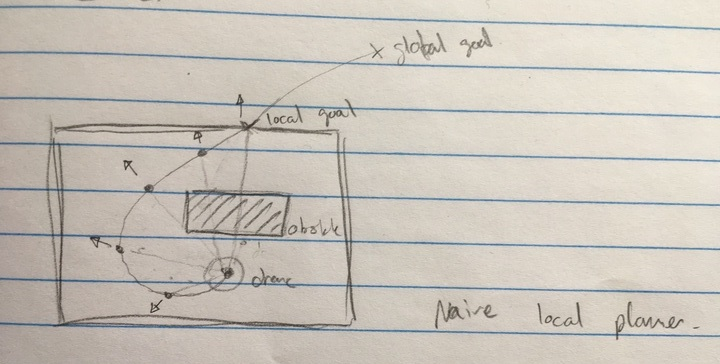
\includegraphics[width=0.9\textwidth]{imgs/sample_global.jpg}
        \caption{Sampling global path to generate local trajectories}
    \end{subfigure}%
    \begin{subfigure}{0.33\textwidth}
        \centering
        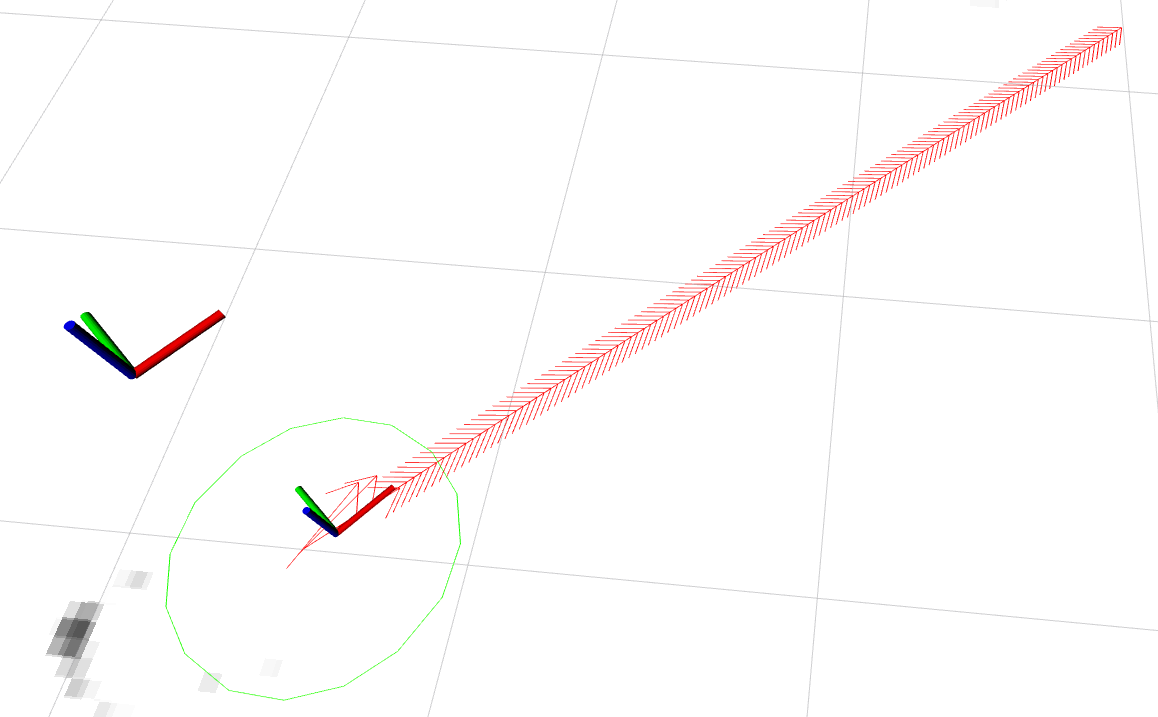
\includegraphics[width=0.9\textwidth]{imgs/one_local_traj.png}
        \caption{Visualization of one local trajectory}
    \end{subfigure}
    \begin{subfigure}{0.33\textwidth}
        \centering
        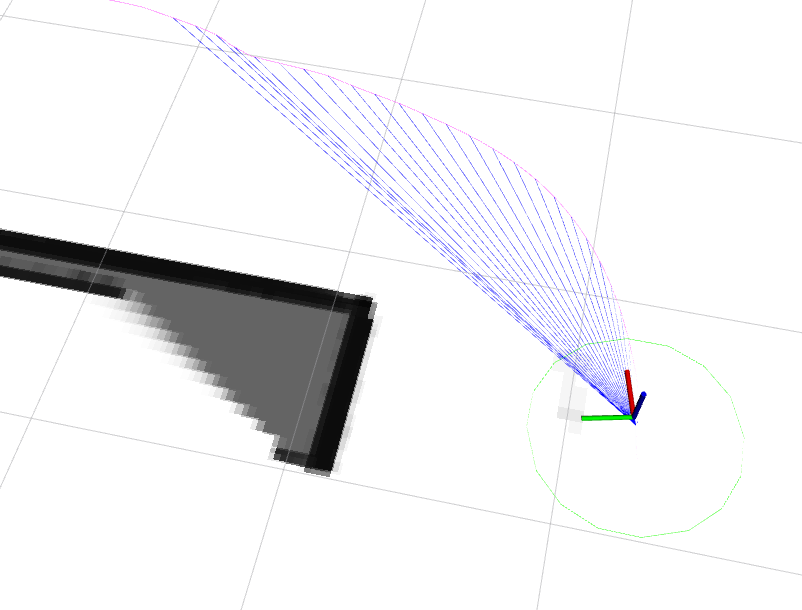
\includegraphics[width=0.9\textwidth]{imgs/local_traj_gen.png}
        \caption{Local trajectory generator}
    \end{subfigure}
    \caption{Local trajectory generation\label{fig:local_traj_gen}}
\end{figure}

This approach performed well in most situations however, there were issues under certain circumstances. \\

When drone was nearby the global target the local goal heading could be up to 180 degrees out of phase with the global goal heading\footnote{https://github.com/ursa-drone/ursa-server/issues/25}.  This is because headings were generated by ‘drawing’ a line between current drone position and local target.  If the drone drifted in front of the global target, the local target would be updated to point in the opposite direction.  This is a critical issue as it would prevent the drone from ever achieving goal position.  To solve this problem only the global path endpoint was used to generate a local trajectory when within some multiplier of the robot footprint.  Therefore the only possible local trajectory was a path to the global plan goal with the same heading.  This resolved the issue.

\begin{figure}[H]
    \centering
    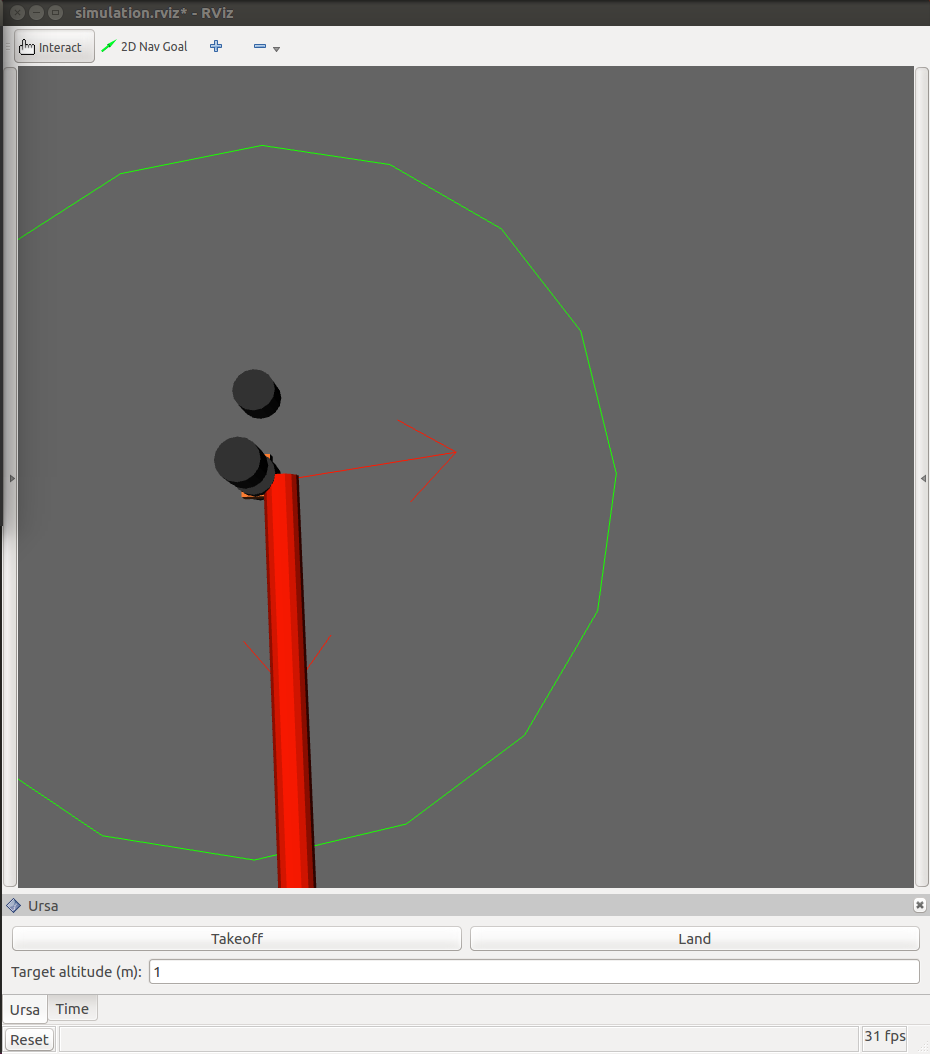
\includegraphics[width=0.4\textwidth]{imgs/out_of_phase.png}
    \caption{Local plan goal out of phase with global plan goal\label{fig:lp_gp_out_of_phase}}
\end{figure}

Another issue was identified when observing the drone turn corners in simulation.  Sampling only along the global path results in a restricted set of potential local paths.  This in turn lead to unsafe close rounding of corners because the global planner always selects the shortest path as discussed above.  There were other factors involved in close rounding of corners, which are covered in the cost functions section below.  To increase the sample space of potential trajectories, points perpendicular to the global plan were added.  These points were set to be some multiplier away from the global plan.  This solution presented the same issue; therefore the length of perpendicular points was set to be a uniform random variable.

\begin{figure}[H]
    \centering
    \begin{subfigure}{0.5\textwidth}
        \centering
        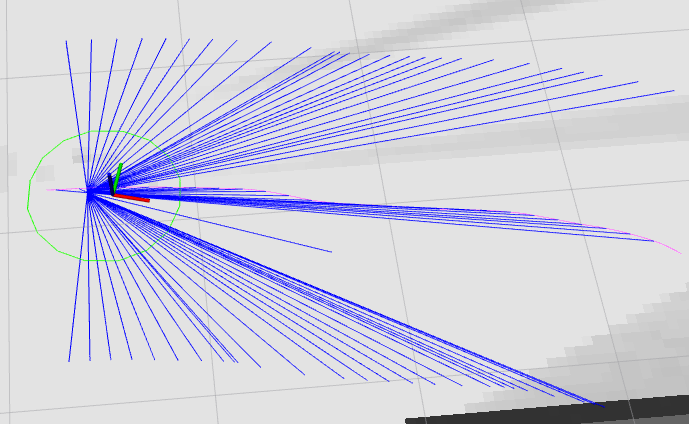
\includegraphics[width=0.9\textwidth]{imgs/local_traj_gen_perp.png}
        \caption{Local trajectories with additional perpendicular points}
    \end{subfigure}%
    \begin{subfigure}{0.5\textwidth}
        \centering
        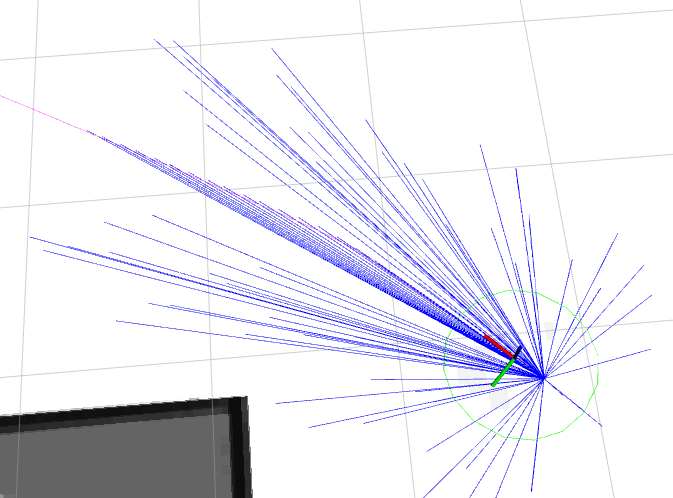
\includegraphics[width=0.9\textwidth]{imgs/local_traj_gen_random.png}
        \caption{Perpendicular points with length as uniform random variable}
    \end{subfigure}
    \caption{Perpendicular points\label{fig:local_traj_gen_perp}}
\end{figure}

Algorithm \ref{alg:trajgen} summarises the operation of the local trajectory generator in pseudocode.\\
\begin{algorithm}[H]
\SetKwInput{KwInput}{Input}
\SetKwInput{KwOutput}{Output}
\KwInput{vector position, vector global\_traj, vector previous\_traj}
\KwOutput{vector samples, vector previous\_traj}
\KwResult{Given current drone position and global plan, output is a vector of 
positional co-ordinates (x,y,th) for use in generating trajectories}\vspace{1.5mm}

\uIf{global\_traj\_endpoint inside radius}{
samples.push(global\_traj.back());
}
\uElse{
\tcc{Add points along the global plan at 10cm intevals}
\For{i in global\_traj}{
    dist = euclidean\_dist(samples.back(), global\_traj[i])\\
    \If{dist $\geq$ 0.1}{
        samples.push(global\_traj[i])
    }
}\vspace{3.5mm}
\tcc{Generate perpendicular points (random length)}
\For{j in samples}{
    samples.push(perp\_points(samples[j]))
}
}\vspace{3.5mm}
\tcc{Add previous trajectory}
\If{previous\_traj}{
samples.push(previous\_traj.back())
}
\caption{Local trajectory sampling of global plan}
\label{alg:trajgen}
\end{algorithm}

\subsubsection{Cost Functions}

In the above section we made the assumption that cost functions had been implemented.  Of course, without the appropriate cost functions no trajectory could be selected, as they would not be distinguishable from one another.  In this section we cover the cost functions utilised by the URSA local planner.  We first consider the desired properties of a local trajectory.  Ideally we want our drone to follow a trajectory that:
\begin{itemize}
    \item Avoids collisions
    \item Give sufficient clearance to obstacles
    \item Advances drone furthest along global path
    \item Ensures drone is facing in direction of movement
\end{itemize}

To achieve these design specifications we modified the ObstacleCostFunction class, added the UrsaGoalCostFunction and made modifications to the dwa local planner.\\

All cost functions must adhere to the TrajectoryCostFunction interface. The TrajectoryCostFunction is again simple, with the most notable requirement being that a score functions follows the format:

\begin{lstlisting}[language=c++]
    virtual double  scoreTrajectory (Trajectory &traj)=0
\end{lstlisting}

For a given trajectory the cost function returns a score which is some double.  By definition negative costs denote a trajectory has passed through an obstacle and low scores indicate a preferable trajectory.  For each trajectory the local planner assigns a score by summing the contributions from each cost function.   In this way the cost functions are modular, with the option of adding or removing costs to suit the implementation.  

\paragraph{Obstacle Cost Function}  
The purpose of the obstacle cost function is to prevent the drone from colliding with obstacles.  After minor modifications to this function and in combination with the UrsaGoalCostFunction we were also able to achieve sufficient clearance around obstacles. \\

A core concept to understanding how the obstacle cost function is understanding the local costmap model.  The local costmap is generated in realtime from the laser scan data.  From this it creates two layers; the obstacle map layer and the inflation layer. \\

The obstacle map layer places laser scan data in a two dimensional grid.  Cells containing sensor readings are marked as occupied whereas the space between the drone and this reading is marked as clear.\\

The inflation layer creates a buffer around the occupied cells by propagating costs via a decaying exponential.  Sensor readings indicate obstacles, therefore if the centre point of a robot was inside these cells there would definitely be a collision.  Therefore these cells are prescribed the maximum cost 254 and are referred to as lethal costs.  The next two costs are referred to as inscribed and circumscribed costs.  These names refer to how the costmap handles robots of arbitrary shapes.  The circumscribed region of the robot is a circle passing through the outermost points of the robots perimeter.  The inscribed region is a circle passing through the innermost regions of its perimeter (\ref{fig:circumscribed}).  Obstacles within the inscribed region are definitely in collision with the robot, therefore these cells are assigned a score of 253.  In our case the inscribed and circumscribed regions are the same as we approximate our drone shape by a circle.  Cells at a distance further than the circumscribed radius have their costs determined by a decaying exponential function (Figure \ref{fig:inflation_radius}).

\begin{align*}
    cost\_decay &= 252*\exp(-1 * csf * (dist\_obst - radius))\\
    csf &=    \text{cost scaling factor}\\
    dist\_obst &=    \text{distance from drone centre cell to obstacle}
\end{align*}

\begin{figure}[H]
    \centering
    \begin{subfigure}{0.5\textwidth}
        \centering
        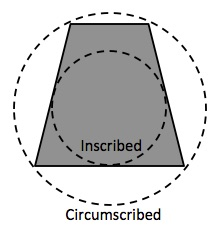
\includegraphics[width=0.65\textwidth]{./imgs/circumscribed.jpg}
        \caption{Circumscribed and inscribed radius}
        \label{fig:circumscribed}
    \end{subfigure}%
    \begin{subfigure}{0.5\textwidth}
        \centering
        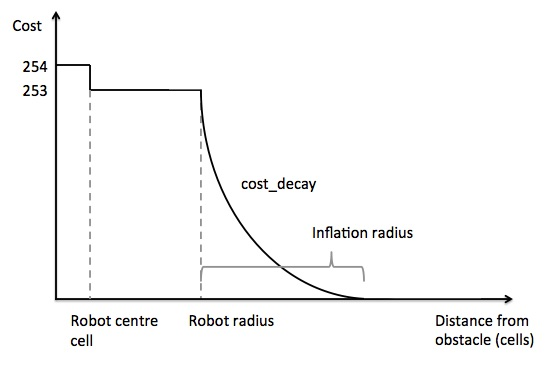
\includegraphics[width=1.1\textwidth]{./imgs/inflation_radius.jpg}
        \caption{Illustration of the inflation radius}
        \label{fig:inflation_radius}
    \end{subfigure}
    \caption{Inflation layer\label{fig:inflation_layer}}
\end{figure}

The exponential function can be tuned using the cost scaling factor and inflation radius parameter.  The cost scaling factor controls the rate at which the costs approach 1.  The inflation radius sets a hard boundary for which the inflation layer extends.  Figure \ref{fig:costmap_config} shows various configurations of the inflation layer.\\

\begin{figure}[H]
    \centering
    \begin{subfigure}{0.33\textwidth}
        \centering
        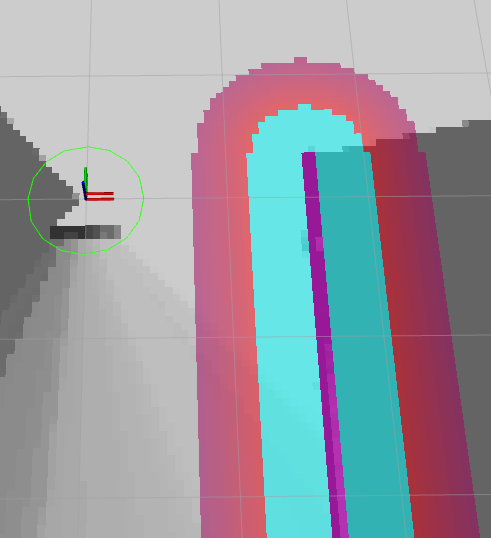
\includegraphics[width=0.9\textwidth]{imgs/lcm/lcm_csf_1_ir_08.png}
        \caption{csf = 1, ir = 0.8}
    \end{subfigure}%
    \begin{subfigure}{0.33\textwidth}
        \centering
        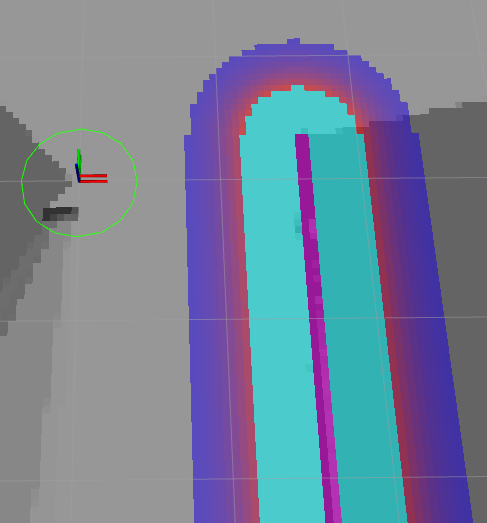
\includegraphics[width=0.9\textwidth]{imgs/lcm/lcm_csf_553_ir_08.png}
        \caption{csf = 5.53, ir = 0.8}
    \end{subfigure}
    \begin{subfigure}{0.33\textwidth}
        \centering
        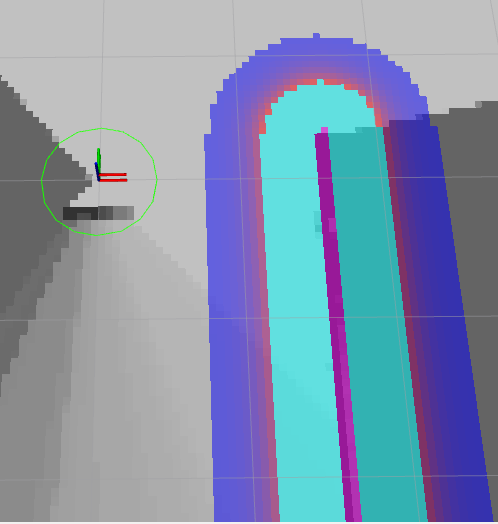
\includegraphics[width=0.9\textwidth]{imgs/lcm/lcm_csf_10_ir_08.png}
        \caption{csf = 10, ir = 0.8}
    \end{subfigure}
        \begin{subfigure}{0.33\textwidth}
        \centering
        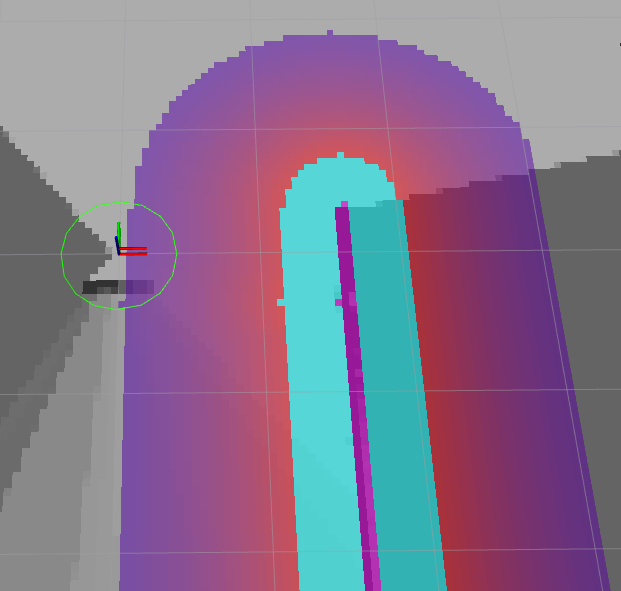
\includegraphics[width=0.9\textwidth]{imgs/lcm/lcm_csf_1_ir_15.png}
        \caption{csf = 1, ir = 1.5}
    \end{subfigure}%
    \begin{subfigure}{0.33\textwidth}
        \centering
        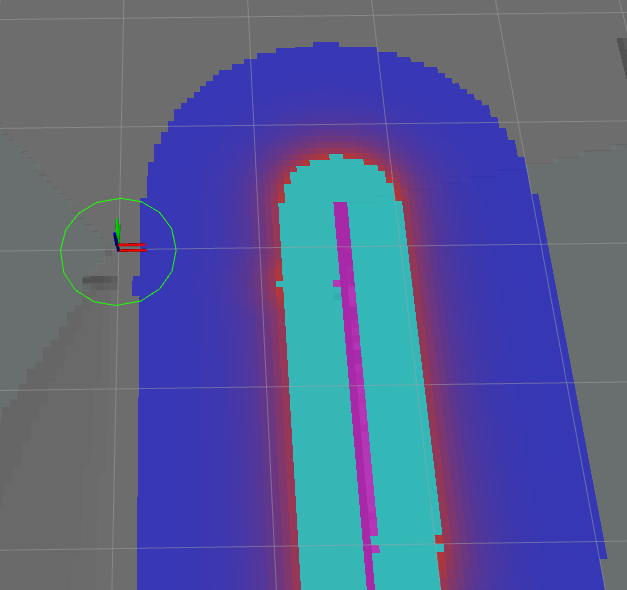
\includegraphics[width=0.9\textwidth]{imgs/lcm/lcm_csf_553_ir_15.png}
        \caption{csf = 5.53, ir = 1.5}
    \end{subfigure}
    \begin{subfigure}{0.33\textwidth}
        \centering
        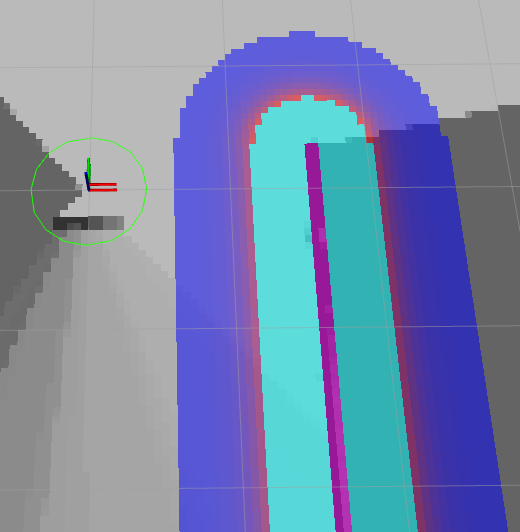
\includegraphics[width=0.9\textwidth]{imgs/lcm/lcm_csf_10_ir_15.png}
        \caption{csf = 10, ir = 1.5}
    \end{subfigure}
    \caption{Various configurations of the cost scaling factor (csf) and inflation radius (ir)}\label{fig:costmap_config}
\end{figure}

The ideal configuration of the costmap could be debated depending on situation and desired properties.  In some instances you may want the drone to take the safest path by preferring to choose paths through the middle of a room.  This could be achieved by setting the inflation radius to a large value so that the whole area is prescribed some cost value.  However, in large indoor areas this may cause our drone to lose its position estimation if the nearest walls our outside its maximum range (5.6m).  In the case that speed to goal is valued it may be preferable to have a smaller inflation radius to result in tighter rounding of corners.  In our implementation we set the inflation radius to be three times the radius.  However, even with this wide buffer, simulation revealed that our drone often opted for paths that merely satisfied the condition of avoiding collisions (Figure \ref{fig:tight_rounding}).  Ideally the behaviour we want is for our drone to prefer local paths furthest from an obstacle.  To implement this we turn to the obstacle cost function.

\begin{figure}[H]
    \centering
    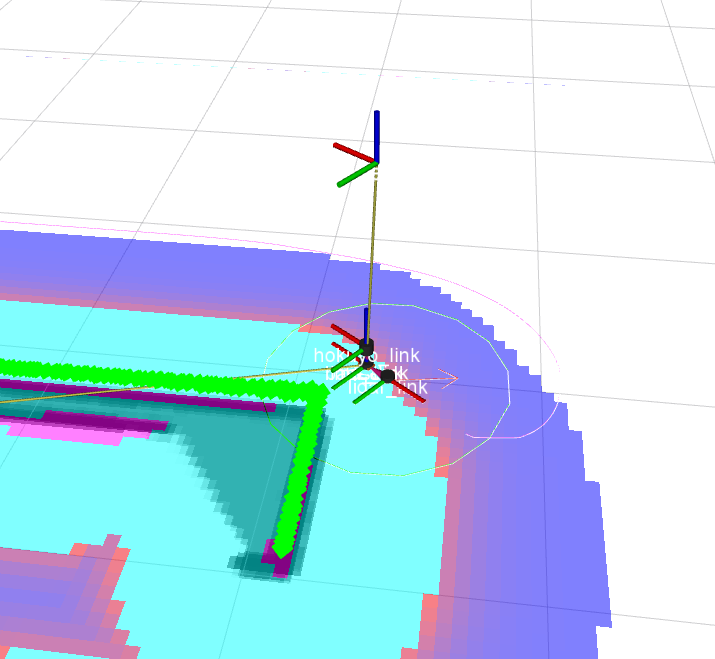
\includegraphics[width=0.4\textwidth]{imgs/does_not_obey_costmap.png}
    \caption{Drone appears to ignore costmap when rounding corners.  Only collision avoidance appears to be satisfied.}\label{fig:tight_rounding}
\end{figure}

Having discussed the workings of costmaps we can now cover how they are utilised by the obstacle cost function to produce a score for local trajectories.  By default the obstacle cost function takes a local trajectory, robot footprint and costmap as inputs and returns a score.  The score is calculated by superimposing the footprint on each point of the local trajectory.  Each footprint passess through a set of cells with some associated cost.  The max of all these sets is the score returned (Figure \ref{fig:ocf_default}). \\

This operation of the obstacle cost function lead to the undesired behaviour of rounding corners too close\footnote{https://github.com/ursa-drone/ursa-server/issues/14}.  Trjectories that pass through lower cost (safe) areas can still receive high costs when taking into account the robots footprint.  Furthermore, all local trajectories have the same origin (robot).  This results in the same cost for all trajectories if the footprint is near a high cost area.  Modifying the obstacle cost function to only return the footprint cost at the radius of the drone appeared to fix this issue.

\begin{figure}[H]
    \centering
    \begin{subfigure}{0.5\textwidth}
        \centering
        \includegraphics[width=0.9\textwidth]{example-image-a}
        \caption{Default}
        \label{fig:ocf_default}
    \end{subfigure}%
    \begin{subfigure}{0.5\textwidth}
        \centering
        \includegraphics[width=0.9\textwidth]{example-image-a}
        \caption{Modified}
        \label{fig:ocf_mod}
    \end{subfigure}
    \caption{Behaviour of obstacle cost function before and after modification}\label{fig:ocf_comp}
\end{figure}

\paragraph{Ursa goal Cost Function}
The obstacle cost function has encoded our desired behaviour for the drone to avoid obstacles and give sufficient clearance.  If we solely relied on this cost function, no trajectories would be preferred when outside the inflation radius.
Another important specification is for the chosen local trajectory to advance the drone furthest along the global plan.\\

To achieve this Euclidean distance was calculated between the local trajectory endpoint and each point on the global path.  The smallest distance was used to identify the corresponding index along the global path.  A value between 1 and 0 was constructed from this index.  A value of 1 indicated local paths that made no progress along the global path.  A value of 0 indicated that the local plan endpoint was closest to the global plan endpoint.  These values adhere to the assumed operation of cost function prescribing a low score to the most desirable paths.

\begin{figure}[H]
    \centering
    \includegraphics[width=0.4\textwidth]{example-image-a}
    \caption{Operation of Ursa goal cost function}\label{fig:ugcf}
\end{figure}

As mentioned above a final score for a local trajectory is determined by summing across all cost functions.  Therefore, the relative scaling between the obstacle cost function and ursa goal cost encodes some implicit preference between distance from obstacle and length of path.  The most desired behaviour being a trajectory that advances furthest along the global plan whilst being far from obstacles.  The least desired behaviour being a trajectory that does not advance very far along the global plan and is set close to obstacles.  The difficulty is in choosing the trade-off between path length and distance from obstacles.  Multiple attempts were taken to design alternative cost functions to better control desired behaviour \footnote{See local\_costmap\_slider.m}.  However the most robust approach was to include a multiplier in the Ursa goal cost function.  By manipulating this multiplier in simulation acceptable behaviour was found.

\paragraph{Turn Before Moving}
Another desired behaviour for our drone is that it is facing the direction it moves.  There are two main reasons for this.  Firstly the laser scanner used only has 240$^\circ$ field of view.  If travelling in the direction of its blind spot there would be nothing preventing collision with obstacles.  Another important factor is the usage of the onboard camera.  Although not used in any position estimation algorithms the camera gives the operator the ability to remotely retrieve images from the environment.\\

Originally the turn before moving logic was encoded in the cost functions.  This approach required the generation of local trajectories at the origin of the robot and facing in the direction of the global plan.  A cost function then had to be written to favour trajectories pointing within some epsilon of the global plan heading.  This approach turned out to be complicated to implement and somewhat unreliable.  Instead trajectories were generated as described in section \ref{sec: traj_gen}.  If the drone was not heading along the global plan the origin of the local trajectory was published.  Recall that trajectories are merely ordered lists made up of positional coordinates (x,y,th).  Therefore the origin corresponds to the current position of the drone with a heading in the direction of the global path.  When the drone has the correct heading the end point of the local trajectory is published.

\begin{figure}[H]
    \centering
    \begin{subfigure}{0.5\textwidth}
        \centering
        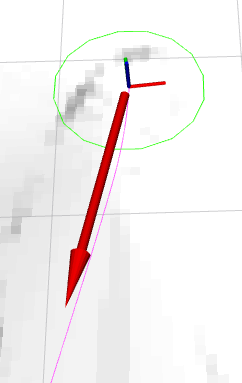
\includegraphics[width=0.9\textwidth]{imgs/tbm_not_facing_target.png}
        \caption{Not facing global plan}
        \label{fig:tbm_not_heading_towards_global}
    \end{subfigure}%
    \begin{subfigure}{0.5\textwidth}
        \centering
        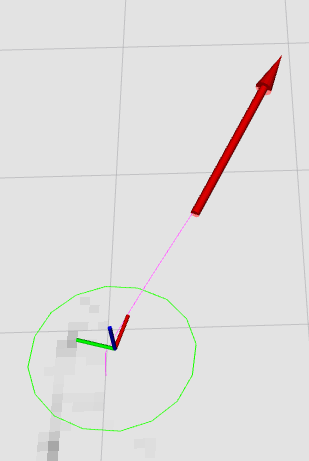
\includegraphics[width=0.9\textwidth]{imgs/tbm_facing_target.png}
        \caption{Facing global plan}
        \label{fig:tbm_heading_towards_global}
    \end{subfigure}
    \caption{Local target for different headings of drone with respect to global path.  Red arrow indicates navigation goal sent to PX4.}\label{fig:tbm}
\end{figure}

\end{document}